\documentclass{article}
\usepackage[utf8]{inputenc}
\usepackage{setspace}
\usepackage{tikz}
\usetikzlibrary{positioning}
\usepackage{amsfonts}
\usepackage{amssymb}
\usepackage{amsmath}
\usepackage{amsthm}
\usepackage{systeme}
\usepackage{mathtools}
\usepackage{hyperref}
\usepackage{venndiagram}
\usepackage{pgfplots}
\usetikzlibrary{pgfplots.statistics}
\pgfplotsset{compat=newest}
\usepackage{logicproof}
\usepackage{mathrsfs}
\allowdisplaybreaks
\usepackage{mathpartir}
\usepackage{graphicx}

\begin{document}
\section*{Question 1}

~

\subsection*{a}

~

\begin{proof}
    \begin{align*}
        &x=m^2-n^2\\
        &y=2mn\\
        &z=m^2+n^2\\
        &x^2+y^2=(m^2-n^2)^2+(2mn)^2\\
        &=m^4-2m^2n^2+n^4+4m^2n^2\\
        &=m^4+2m^2n^2+n^4\\
        &=(m^2+n^2)^2\\
        &=z^2\\
        \Rightarrow&x^2+y^2=z^2\\
        &\\
        &\Rightarrow\\
        &\text{Suppose}:(x,y,z)\text{ are primitive triple}\\
        \Rightarrow&x,y,z\text{ are pairwise co-prime}\\
        &\text{Suppose}: m,n\text{ are not co-prime or both odd}\\
        &\text{case }1:\text{not co-prime}\\
        &\exists p,q,k\ne1\in\mathbb{Z}:m=pk,n=qk\\
        &x=m^2-n^2=(pk)^2-(qk)^2=(p^2-q^2)k^2\\
        &y=2mn=2pk\cdot qk=2pqk^2\\
        &\gcd(x,y)\geqslant k^2>1\\
        \Rightarrow&x,y\text{ are not co-prime}\nLeftrightarrow\\
        &\text{case }2:\text{both odd}\\
        &\exists a,b\in\mathbb{Z}:m=2a+1,n=2b+1\\
        &x=m^2-n^2=(2a+1)^2-(2b+1)^2=4a^2+4a-4b^2-4b=4(a^2+a-b^2-b)\\
        &y=2mn=2(2a+1)(2b+1)\\
        &\gcd(x,y)\geqslant 2>1\\
        \Rightarrow&x,y\text{ are not co-prime}\nLeftrightarrow\\
        \Rightarrow&(x,y,z)\text{ are primitive triple}\implies m,n\text{ are co-prime and not both odd}\\
        &\\
        &\Leftarrow\\
        &\text{Suppose}: m,n\text{ are co-prime and not both odd}\\
        &\text{Without loss of generality, suppose}: \exists p,q\in\mathbb{Z}: m=2p,n=2q+1,\gcd(2p,2q+1)=1\\
        &\text{Suppose}: x,y,z\text{ are not pairwise co-prime}\\
        &\text{case }1:\gcd(x,y)>1\\
        &a\coloneqq\gcd(x,y)\\
        \Rightarrow&a|2mn\\
        &a|2\lor a|m\lor a|n\\
        &a \not| 2\text{ since }m,n\text{ are not both even}\\
        &a |m:\\
        &a|m^2-n^2\\
        \Rightarrow&a|n^2\\
        \Rightarrow&a|n\\
        \Rightarrow&\gcd(m,n)\geqslant a>1\nLeftrightarrow\gcd(m,n)=1\\
        &a|n\text{ same condition as }a|m\\
        &\text{case 2}:\gcd(x,z)>1\\
        &a\coloneqq \gcd(x,z)\\
        \Rightarrow&a|m^2-n^2\land a|m^2+n^2\\
        &a|2m^2\land a|2n^2\\
        \Rightarrow&a|2\lor (a|m^2\land a|n^2)\\
        &a\not|2\text{ since }m,n\text{ are not both even}\\
        \Rightarrow&a|m^2\land a|n^2\\
        &a|m\land a|n\\
        \Rightarrow&\gcd(m,n)\geqslant a>1\nLeftrightarrow\gcd(m,n)=1\\
        &\text{case 3}:\gcd(y,z)>1\\
        &a\coloneqq\gcd(y,z)\\
        \Rightarrow&a|2mn\\
        &a|2\lor a|m\lor a|n\\
        &a \not| 2\text{ since }m,n\text{ are not both even}\\
        &a |m:\\
        &a|m^2+n^2\\
        \Rightarrow&a|n^2\\
        \Rightarrow&a|n\\
        \Rightarrow&\gcd(m,n)\geqslant a>1\nLeftrightarrow\gcd(m,n)=1\\
        &a|n\text{ same condition as }a|m\\
        &\\
        \Rightarrow& m,n\text{ are co-prime and not both odd}\implies(x,y,z)\text{ are primitive triple}\\
        \Rightarrow&m,n\text{ are co-prime and not both odd}\Leftrightarrow(x,y,z)\text{ are primitive triple}\\
    \end{align*}
\end{proof}

~

\subsection*{b}

~

\begin{align*}
    &2mn\text{ must be odd}\\
    \Rightarrow&2mn=24\\
    &x<z\\
    \Rightarrow&x=7,z=25\\
    &x=m^2-n^2,z=m^2+n^2\\
    &x+z=2m^2=32\\
    &m=4\lor m=-4\\
    &m=4:\\
    &2mn=24\\
    &n=3\\
    &m=-4:\\
    &2mn=24\\
    &n=-3\\
    \Rightarrow&(m,n)=(4,3)\lor(-4,-3)\\
\end{align*}

~

\subsection*{c}

~

\begin{align*}
    &(x,y,z)\text{ is pairwise co-prime}\\
    \Rightarrow&\text{without loss of generality}:\exists p,q\in\mathbb{Z}: m=2p,n=2q+1,\gcd(2p,2q+1)=1\\
    &z=m^2+n^2\\
    &=(2p)^2+(2q+1)^2\\
    &=4p^2+4q^2+4q+1\\
    &=2(2p^2+2q^2+2q)+1\\
    &2p^2+2q^2+2q\in\mathbb{Z}\\
    \Rightarrow&2(2p^2+2q^2+2q)+1\text{ is odd}\\
    &z\text{ is odd}\\
    &z\text{ cannot be even}\\
\end{align*}

\newpage

\section*{Question 2}

~

Draw perpendicular line of a line at a given point $A$:

Use compass to draw two arcs by center $A$ intersecting the line, the two intersections are marked as $B$ and $C$. At $B$ and $C$, use compass to draw one arc by each $B$ and $C$ as the center, make sure the two circles containing the two arcs have the same radius and the two arcs intersects at one point, marking $D$, then draw a line crossing $A$ and $D$, line $AD$ is the perpendicular line of the orignal line at $A$.

~

Draw parallel line of a line at a given point $A$:

Use compass to draw an arc by center $A$ intersecting the line, marking $B$. Then use the same distance on the compass to draw an arc by center $B$ intersecting the line at $C$, note that $\angle ABC >90^\circ$. Then use the same distance on the compass to draw an arc by center $C$ intersecting the arc centered by $A$, marking the intersection $D$. Then draw a line crossing $A$ and $D$, then line $AD$ is parallel to $BC$, the original line.

~

\subsection*{a}

~

Draw a line on the paper, and select a point $A$ on the line. Use the compass to record the length $x$, then use $A$ as the start point and mark the endpoint of the compass as $B$, then the segment $AB$ has length $x$. Use the compass to record the length $y$, then use $B$ as the start point and mark the endpoint of the compass in the same direction of $\overrightarrow{AB}$ as $C$, then the segment $BC$ has length $y$ and segment $AC$ has length $x+y$.

~

Draw a line on the paper, and select a point $A$ on the line. Use the compass to record the length $x$, then use $A$ as the start point and mark the endpoint of the compass as $B$, then the segment $AB$ has length $x$. Use the compass to record the length $y$, then use $B$ as the start point and mark the endpoint of the compass in the opposite direction of $\overrightarrow{AB}$ as $C$, then the segment $BC$ has length $y$ and segment $AC$ has length $x-y$.

~

\subsection*{b}

~

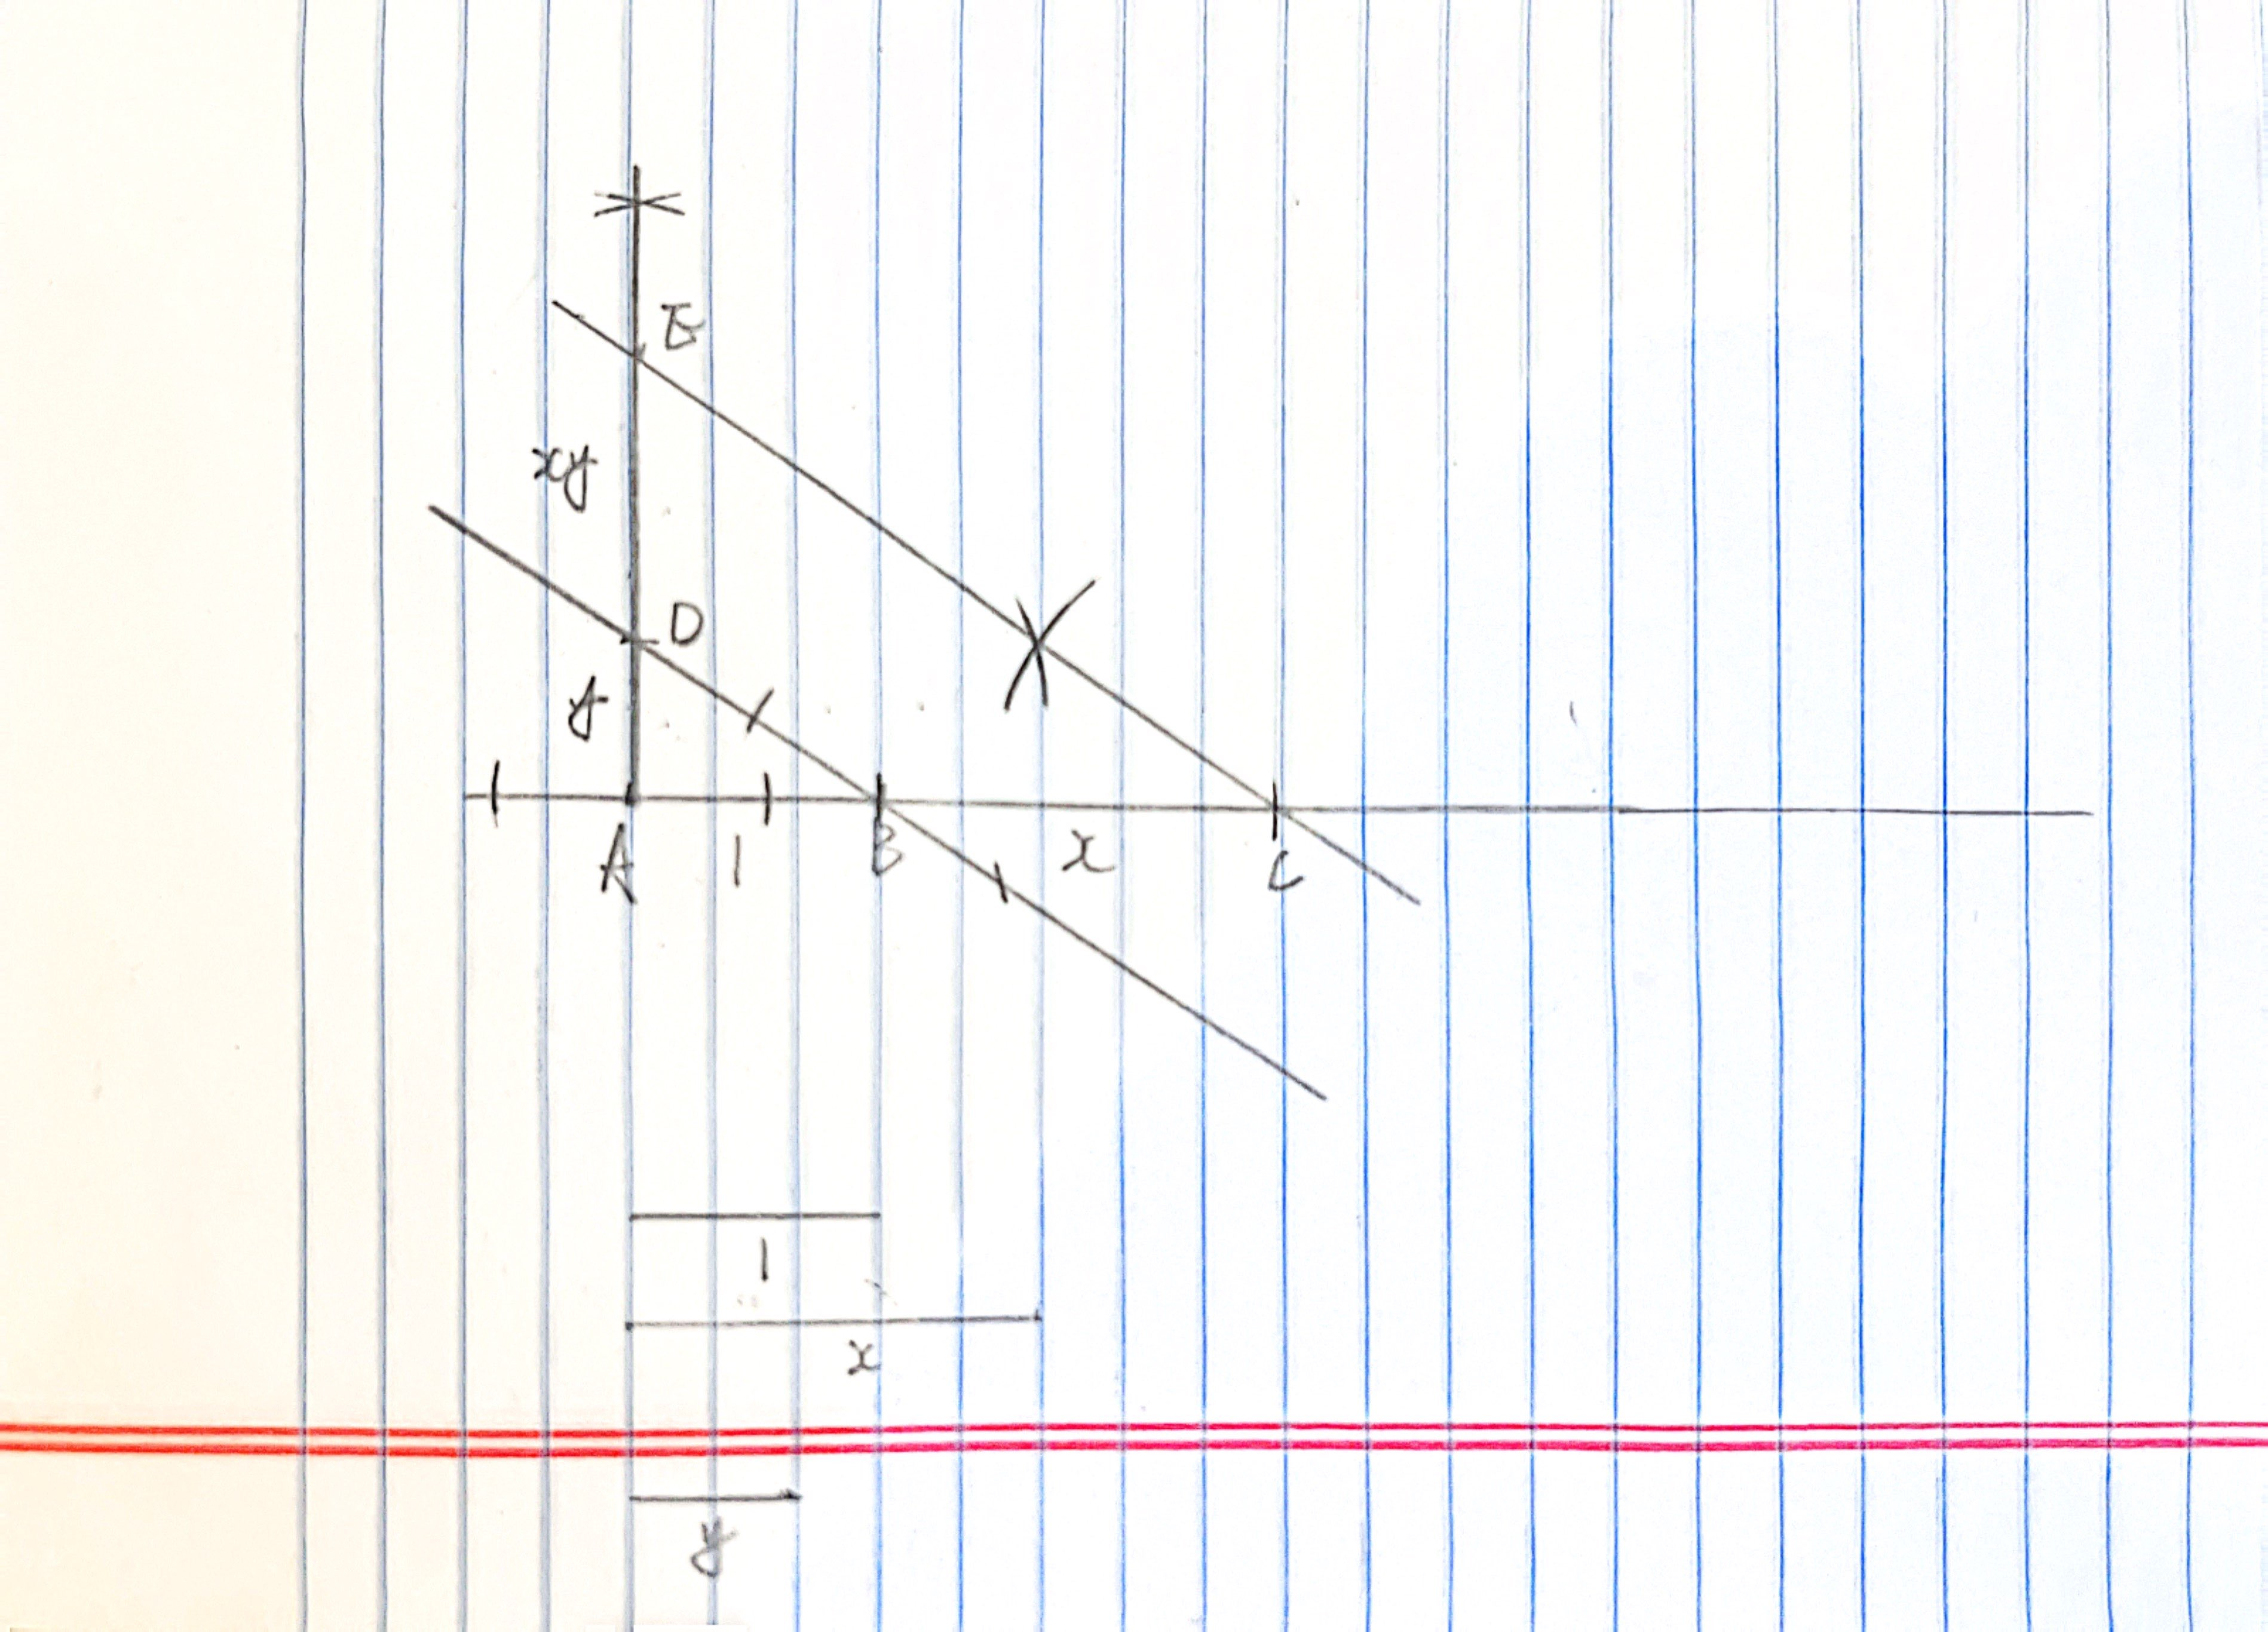
\includegraphics[scale=0.05]{HW_0214/2b_1.jpg}

Draw a line on the paper, and select a point $A$ on the line. Use the compass to record the length 1 and then use $A$ as the start point and mark the endpoint of the compass as $B$, then the segment $AB$ has length $1$. Use the compass to record the length $x$, then use $B$ as the start point and mark the endpoint of the compass in the same direction of $\overrightarrow{AB}$ as $C$, then the segment $BC$ has length $x$. Draw a perpendicular line of the line $AC$ at point $A$. Use the compass to record the length $y$, then use $A$ as the start point and mark the endpoint of the compass on the perpendicular line as $D$, then the segment $AD$ has length $y$ and connect $BD$. At point $C$, draw a line parallel to $BD$, and intersects line $AD$ at $E$, then line segment $DE$ has length $xy$.

~

\subsection*{c}

~

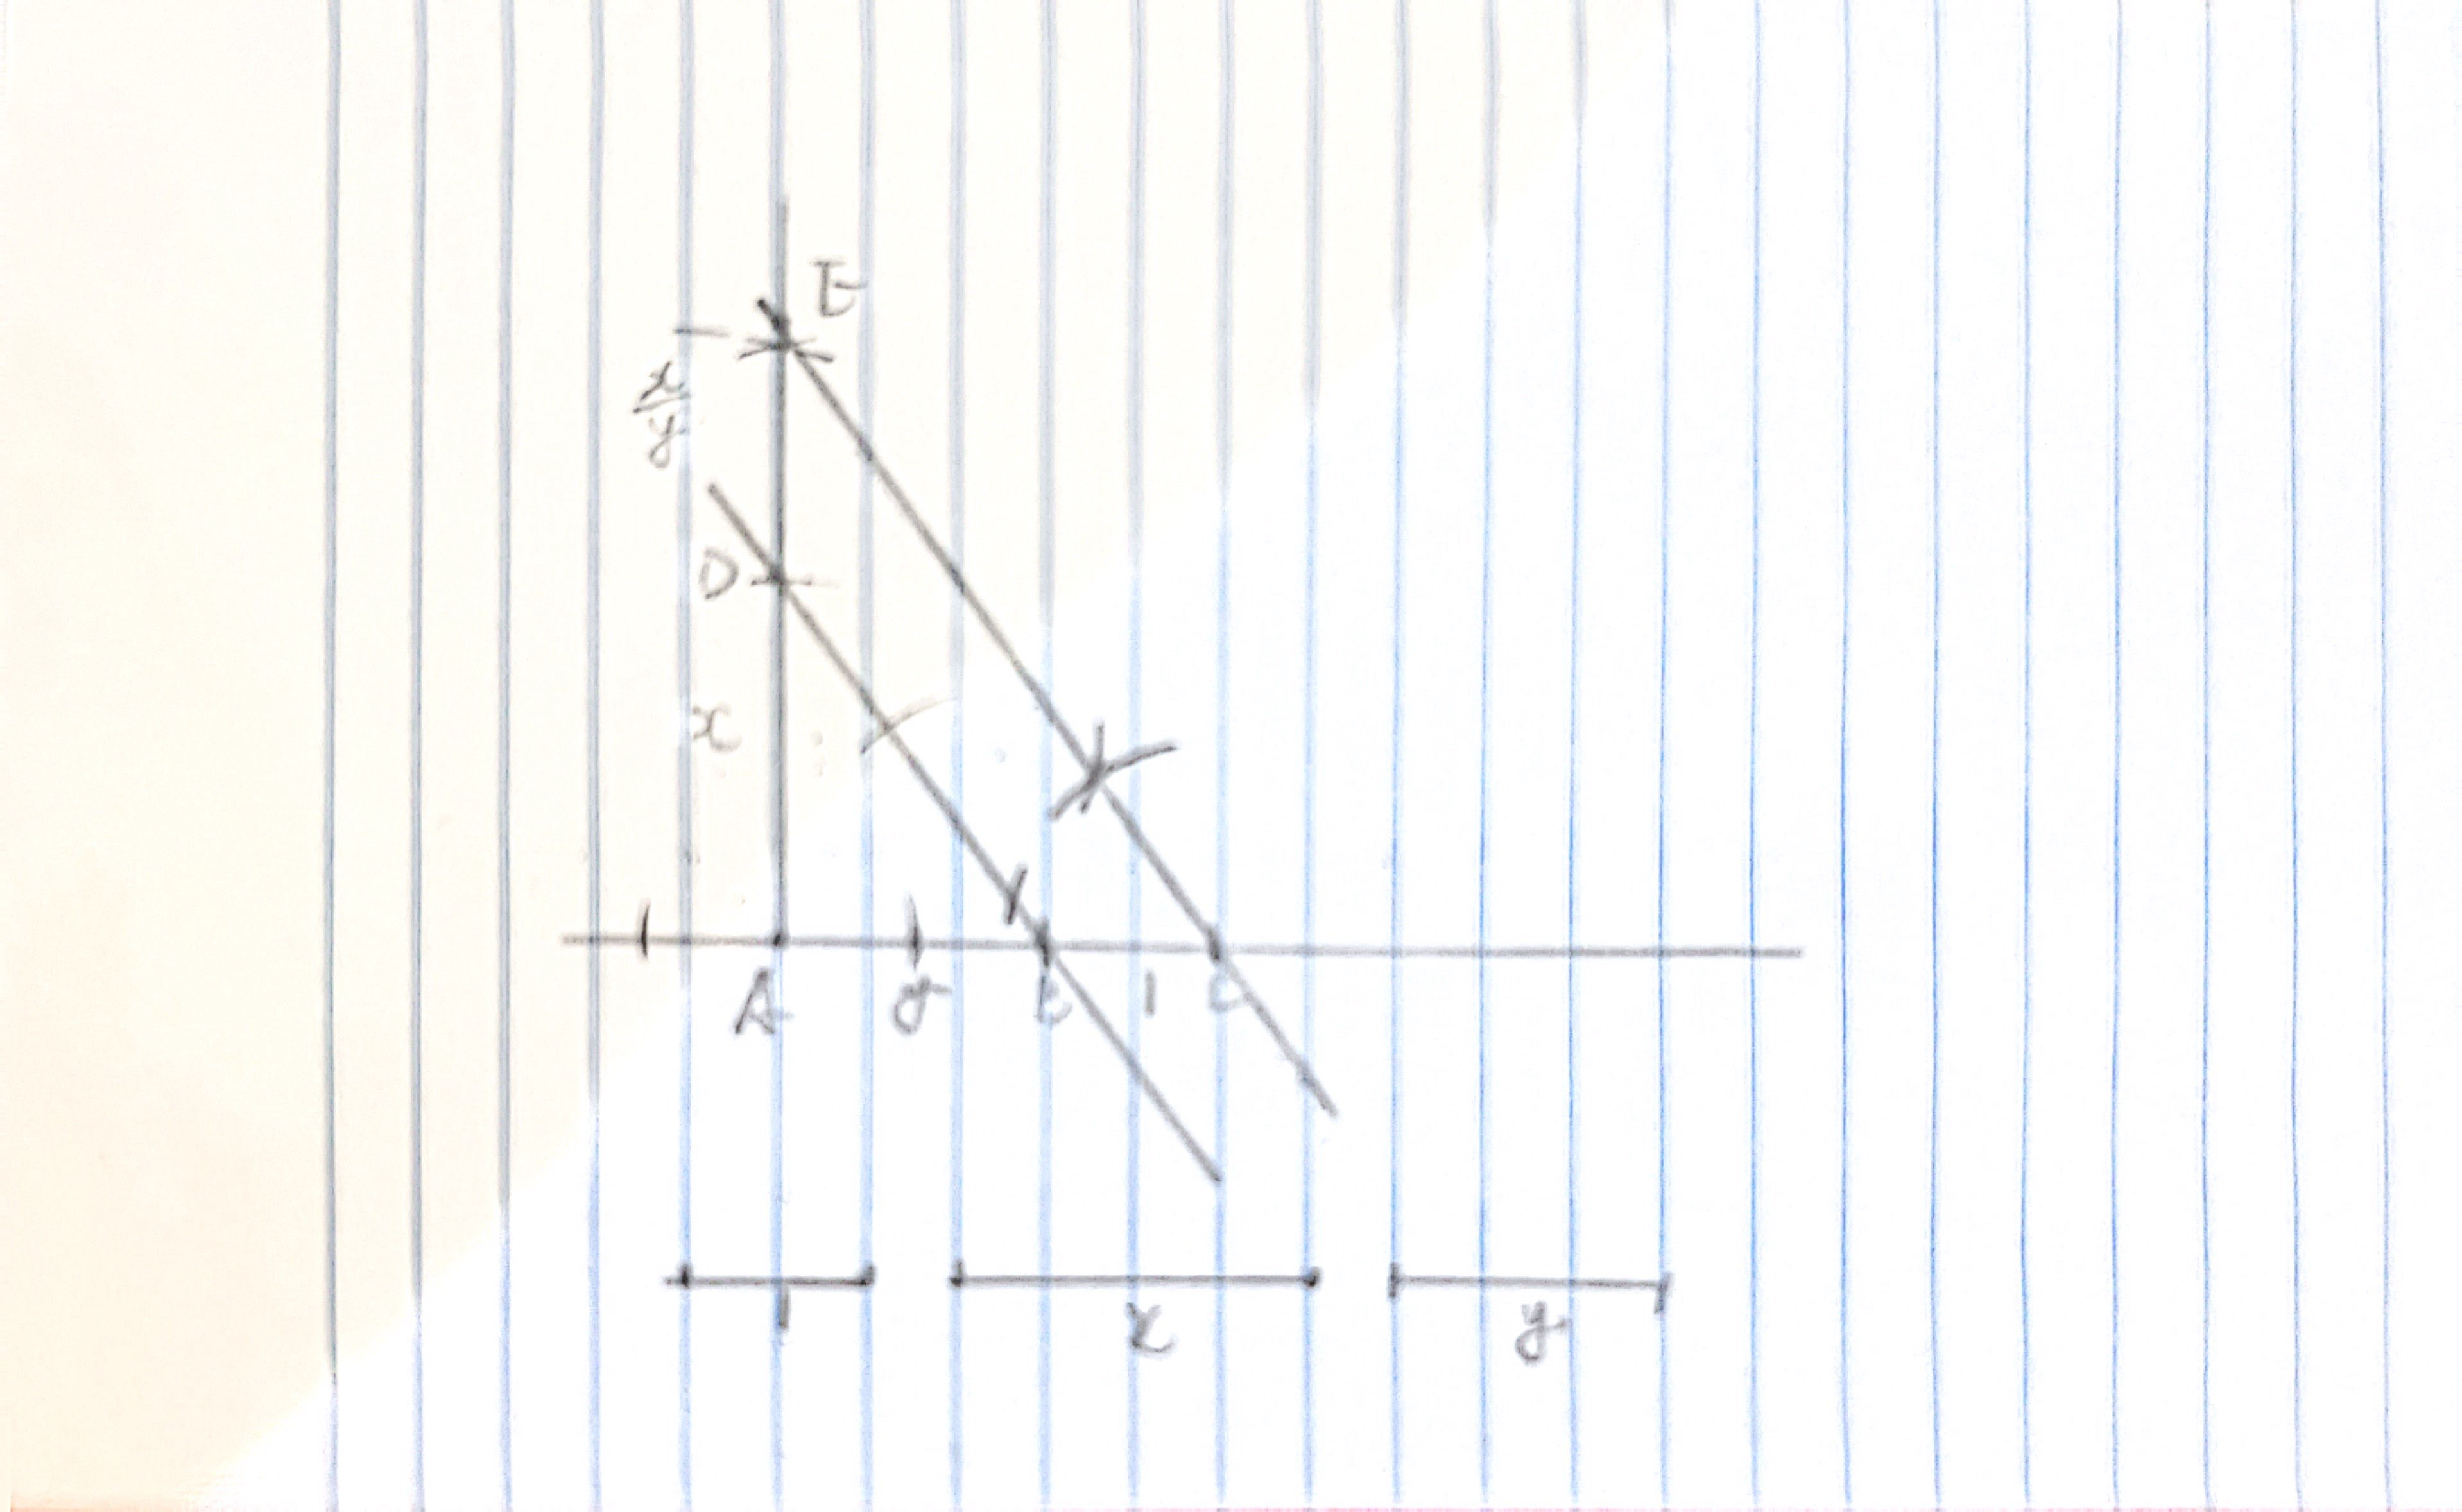
\includegraphics[scale=0.05]{HW_0214/2c_1.jpg}

Draw a line on the paper, and select a point $A$ on the line. Use the compass to record the length $y$ and then use $A$ as the start point and mark the endpoint of the compass as $B$, then the segment $AB$ has length $y$. Use the compass to record the length $1$, then use $B$ as the start point and mark the endpoint of the compass in the same direction of $\overrightarrow{AB}$ as $C$, then the segment $BC$ has length $1$. Draw a perpendicular line of the line $AC$ at point $A$. Use the compass to record the length $x$, then use $A$ as the start point and mark the endpoint of the compass on the perpendicular line as $D$, then the segment $AD$ has length $x$ and connect $BD$. At point $C$, draw a line parallel to $BD$, and intersects line $AD$ at $E$, then line segment $DE$ has length $\frac{x}{y}$.

~

\subsection*{d}

~

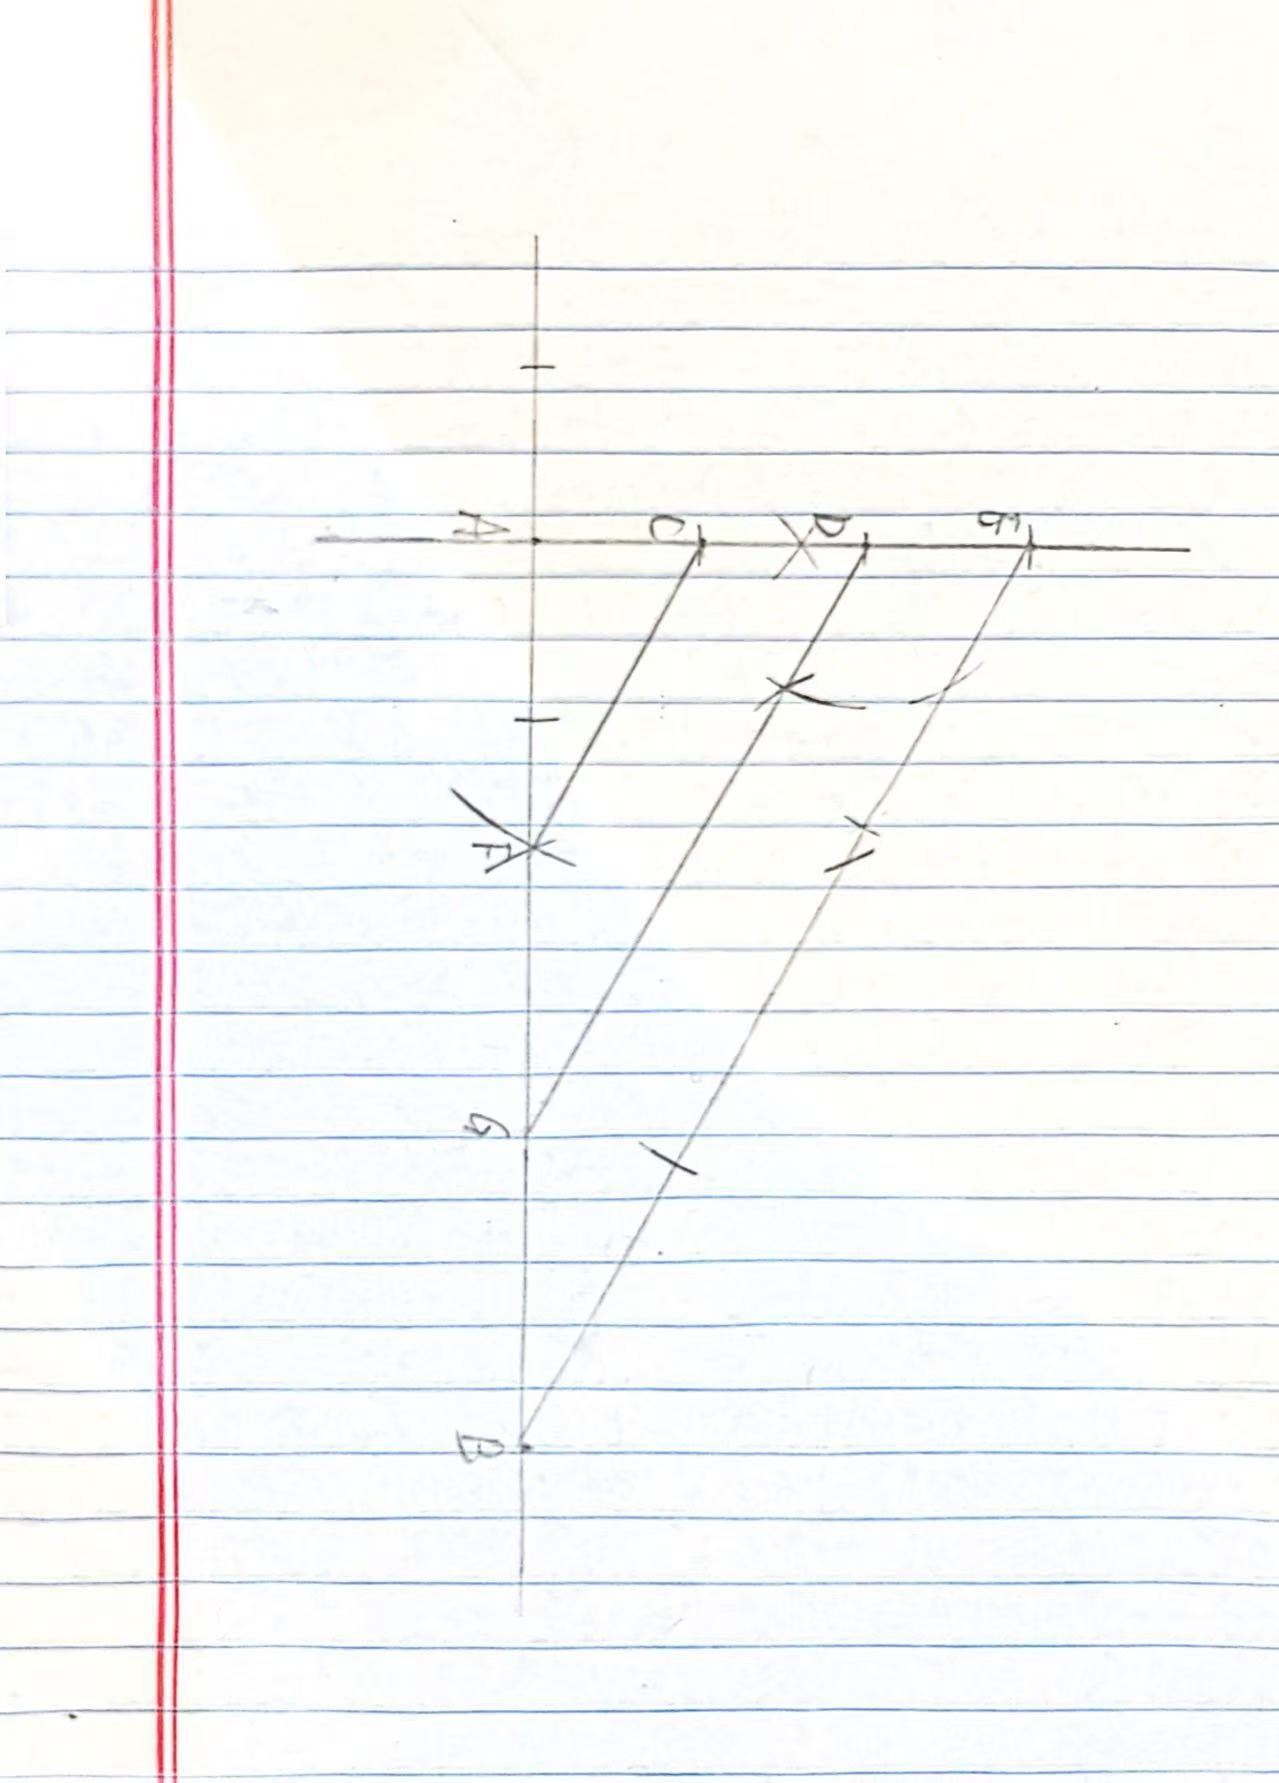
\includegraphics[scale=0.1]{HW_0214/2dre.jpg}

To triply divide a line segment of length $x$, draw a line on the paper, and select a point $A$ on the line. Use the compass to record the length $x$ and then use $A$ as the start point and mark the endpoint of the compass as $B$, then the segment $AB$ has length $x$. Draw a perpendicular line of the line $AB$ at point $A$. Use any length to draw a line segment starting at $A$ on the perpendicular line, marking the endpoint $C$, and draw two more line segments with the same length as line segment $AC$ on line $AC$, marking the two endpoints $D$ and $E$. Make sure that $AC=CD=DE$ and $\overrightarrow{AC}$, $\overrightarrow{CD}$, $\overrightarrow{DE}$ have the same direction. Connect $BE$, and draw two lines parallel to $BE$ at $C$ and $D$, intersecting $AB$ at $F$, $G$ separately. Then $AF=FG=GB=\frac{1}{3}AB$.

\newpage

\section*{Question 3}

(i)

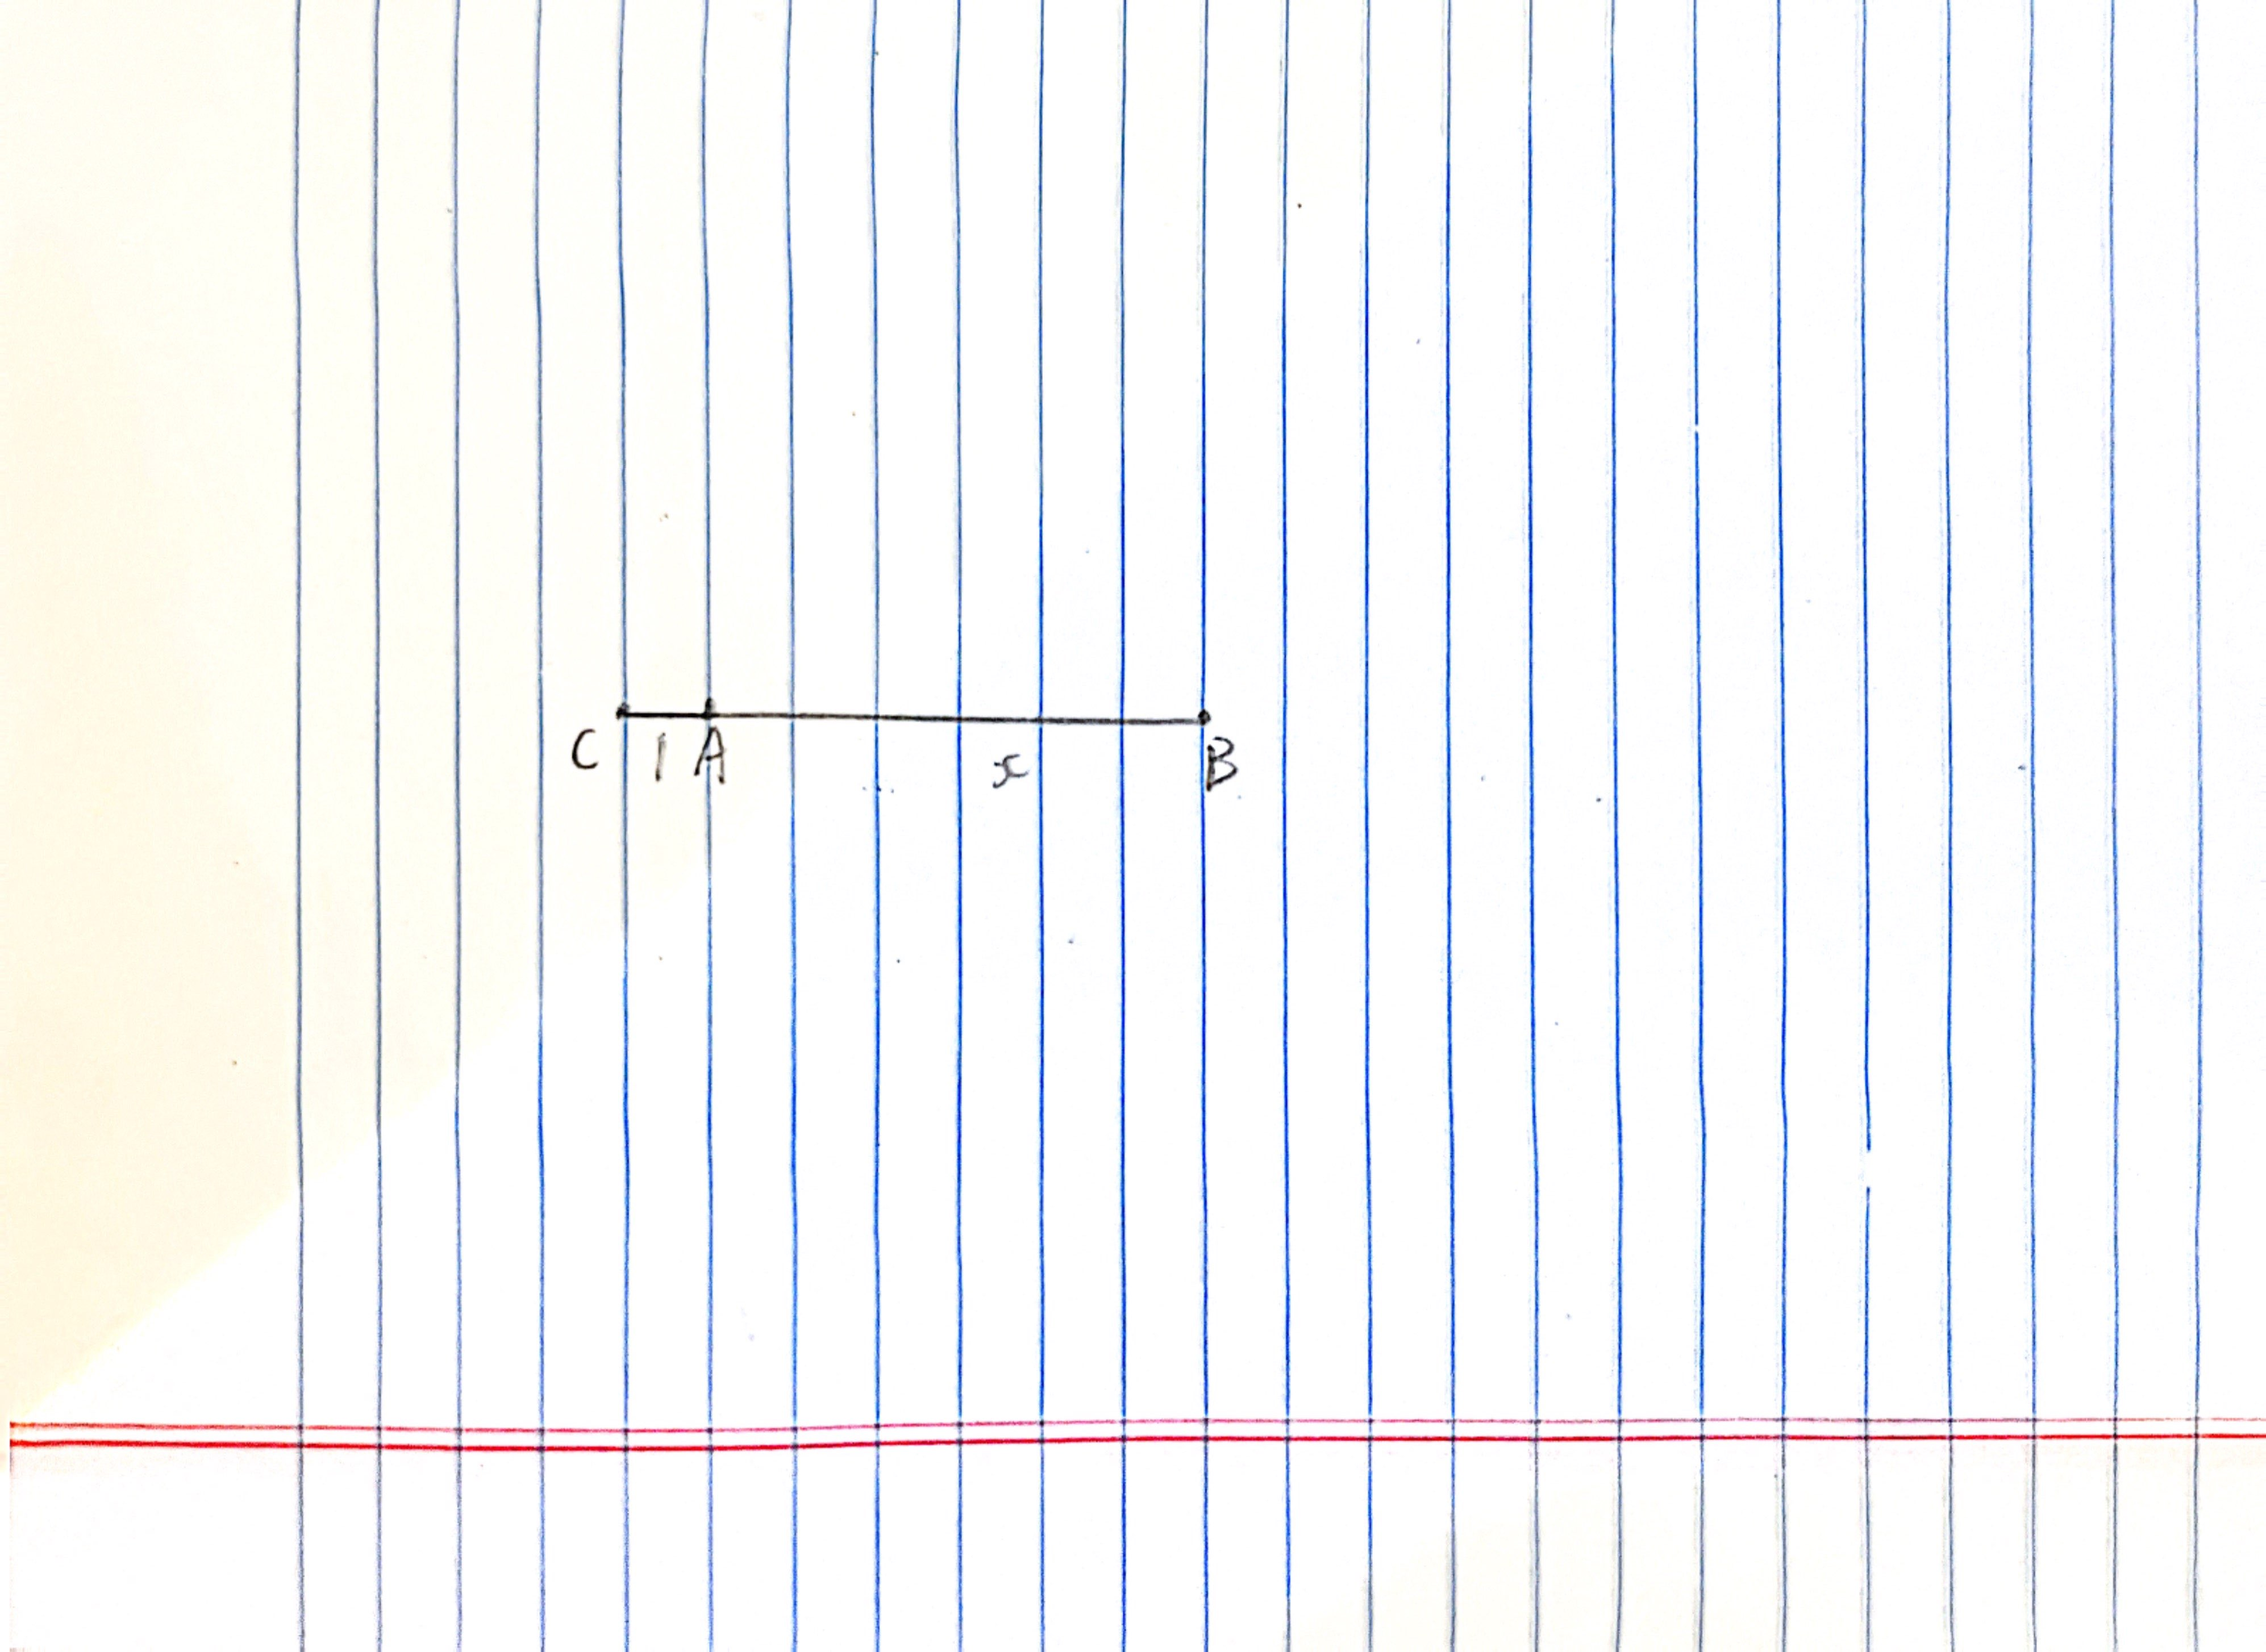
\includegraphics[scale=0.05]{HW_0214/3i_1.jpg}

(ii)

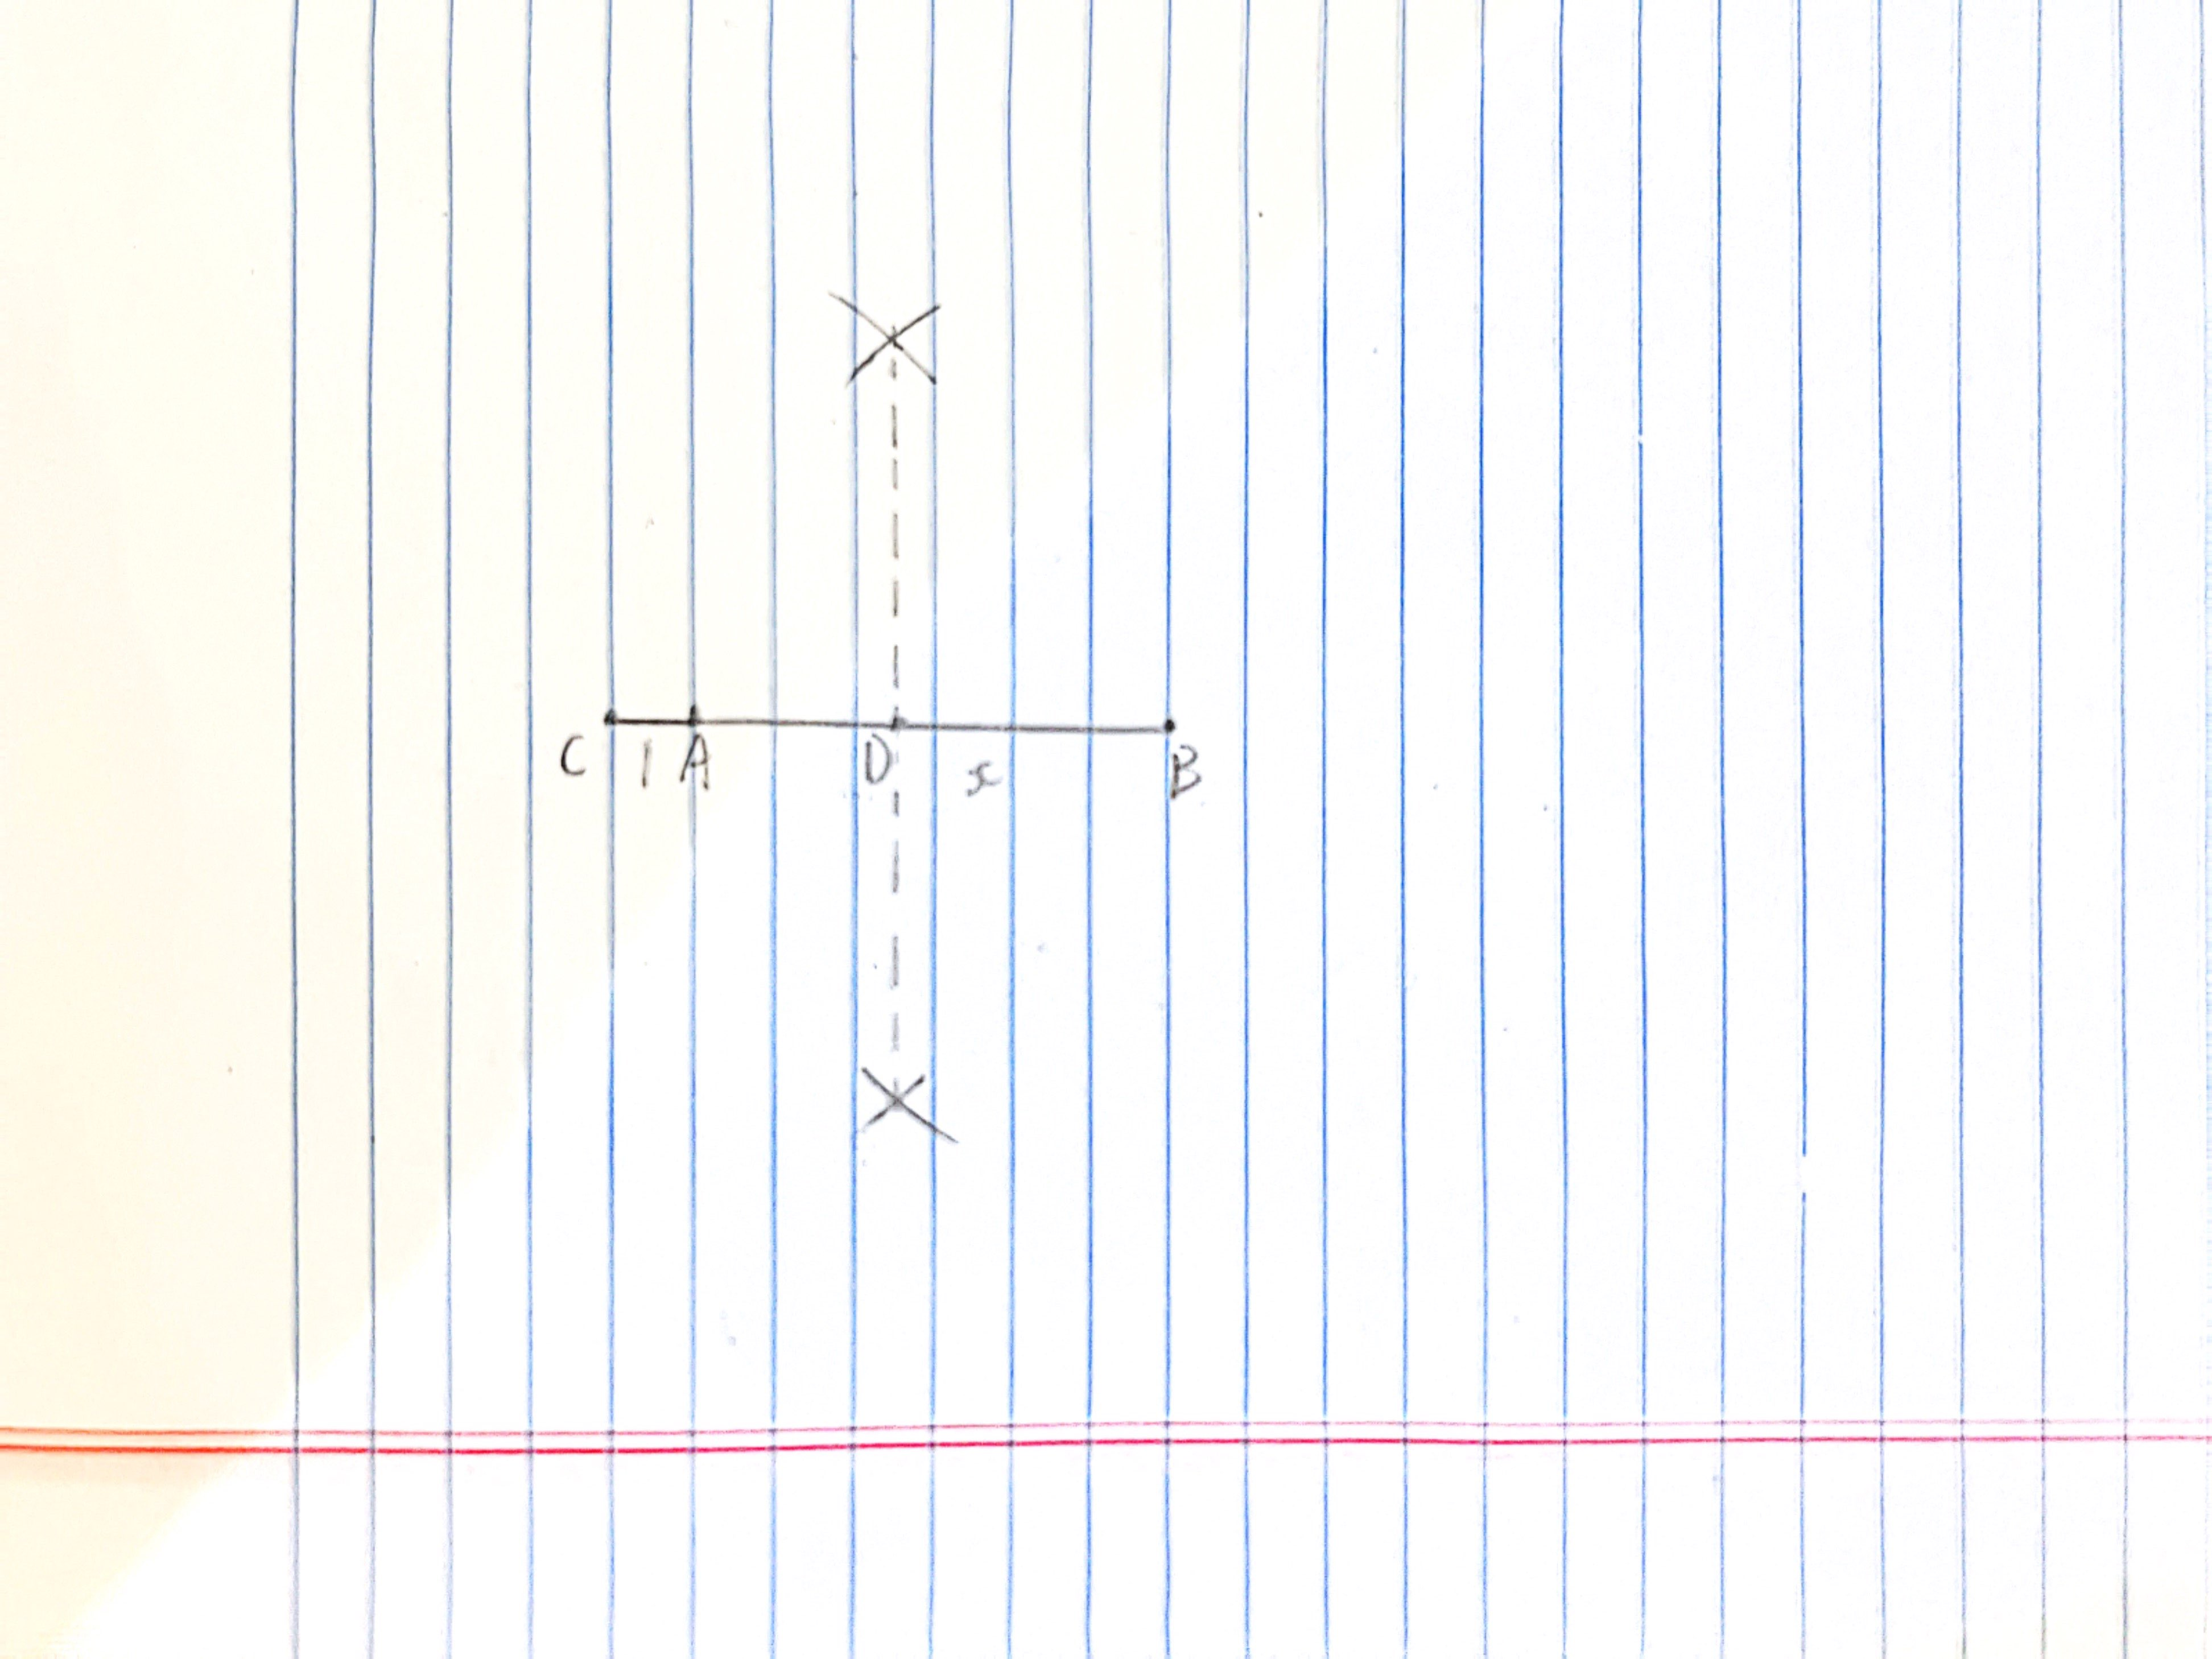
\includegraphics[scale=0.05]{HW_0214/3ii_1.jpg}

(iii)

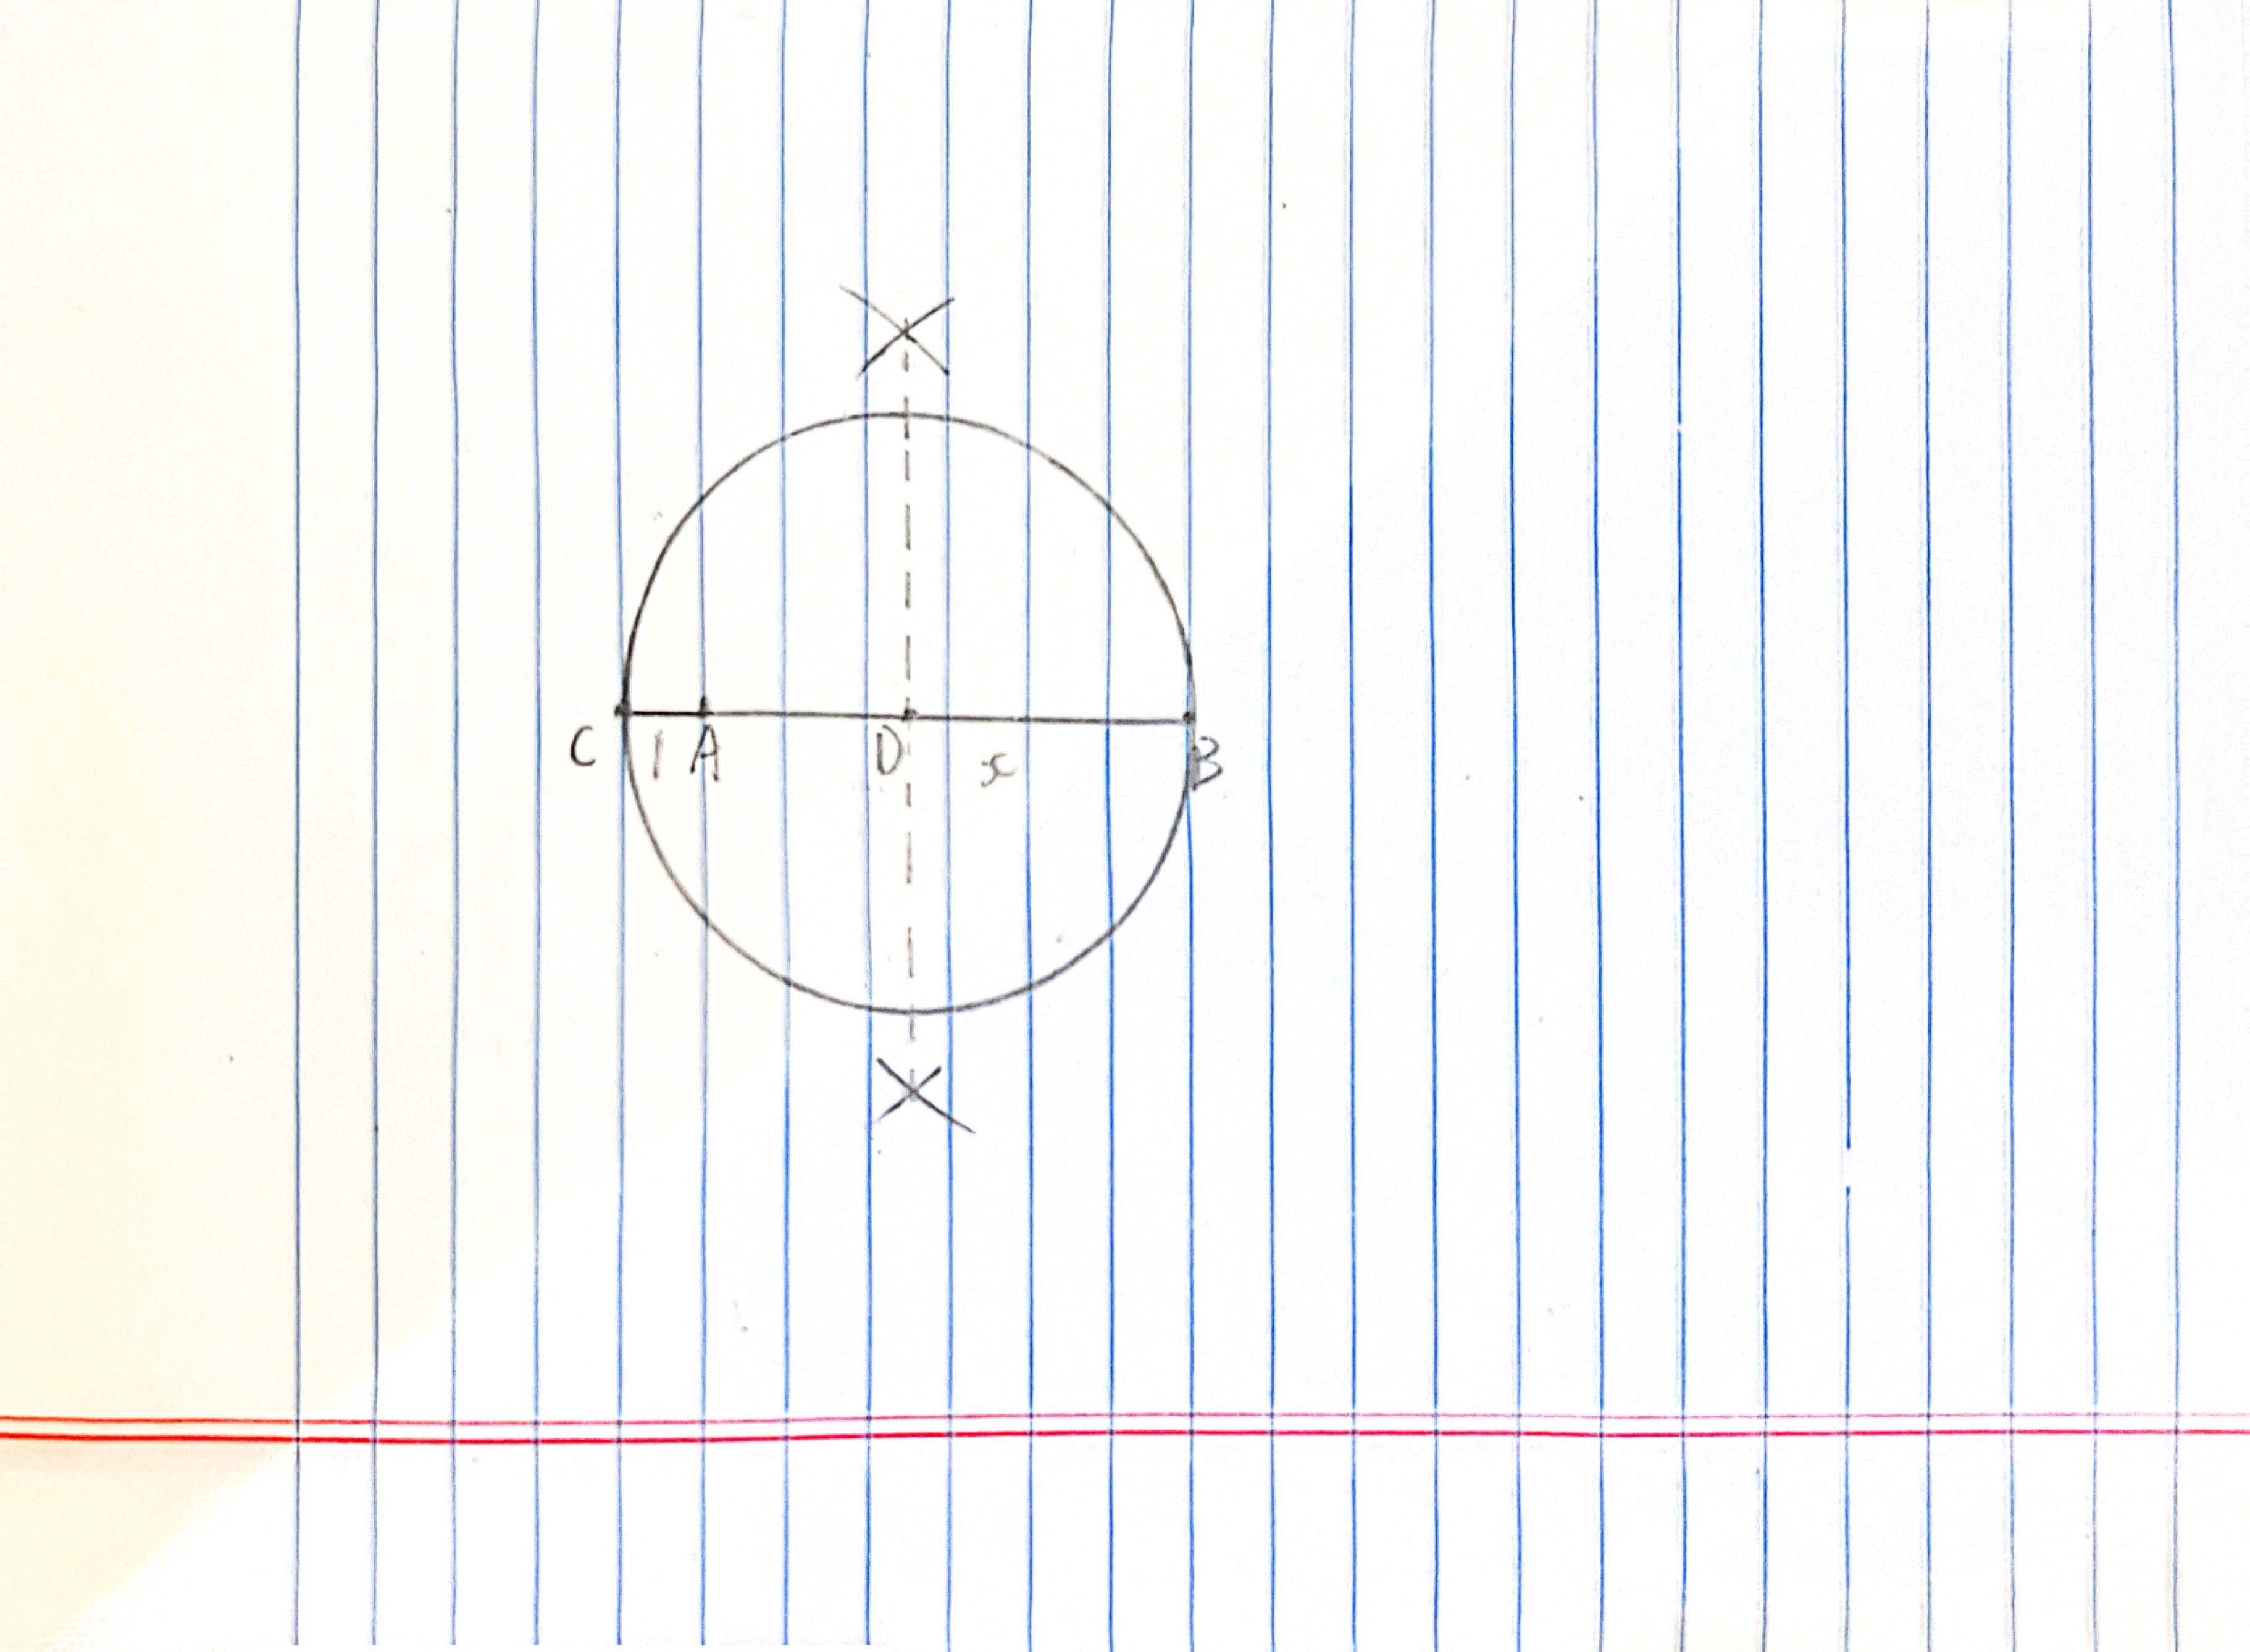
\includegraphics[scale=0.05]{HW_0214/3iii_1.jpg}

(iv)

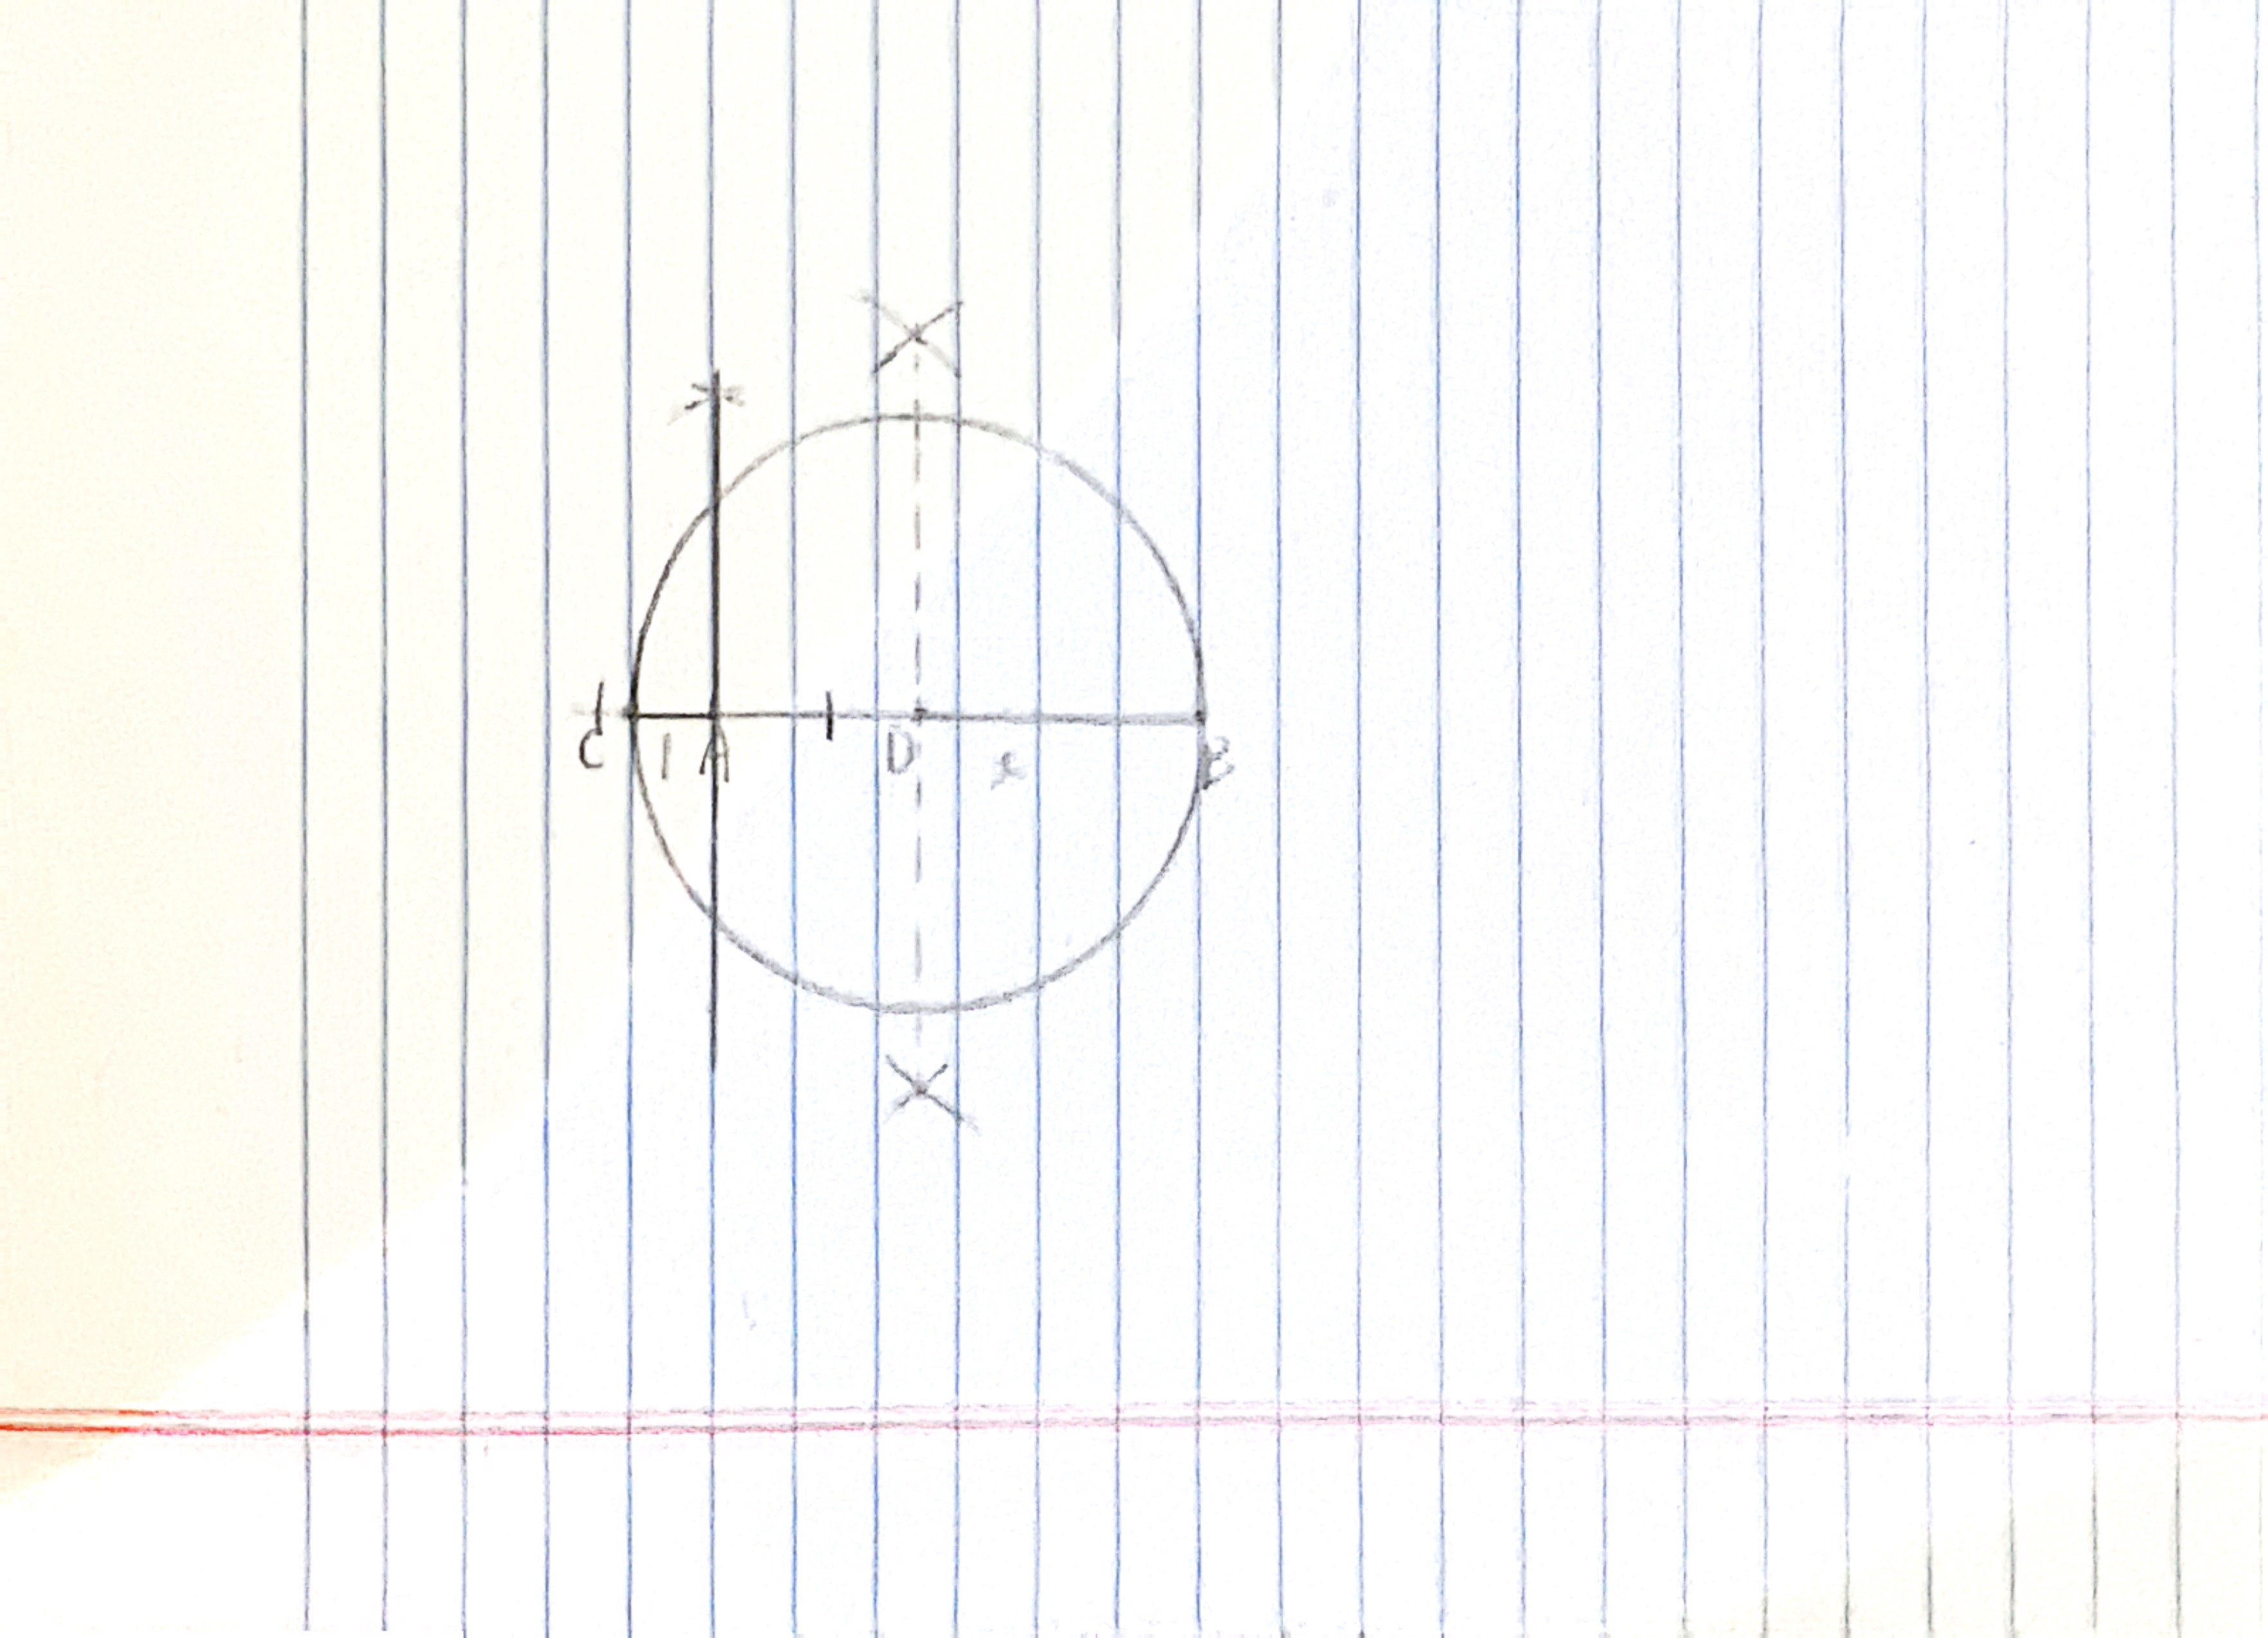
\includegraphics[scale=0.05]{HW_0214/3iv_1.jpg}

(v)

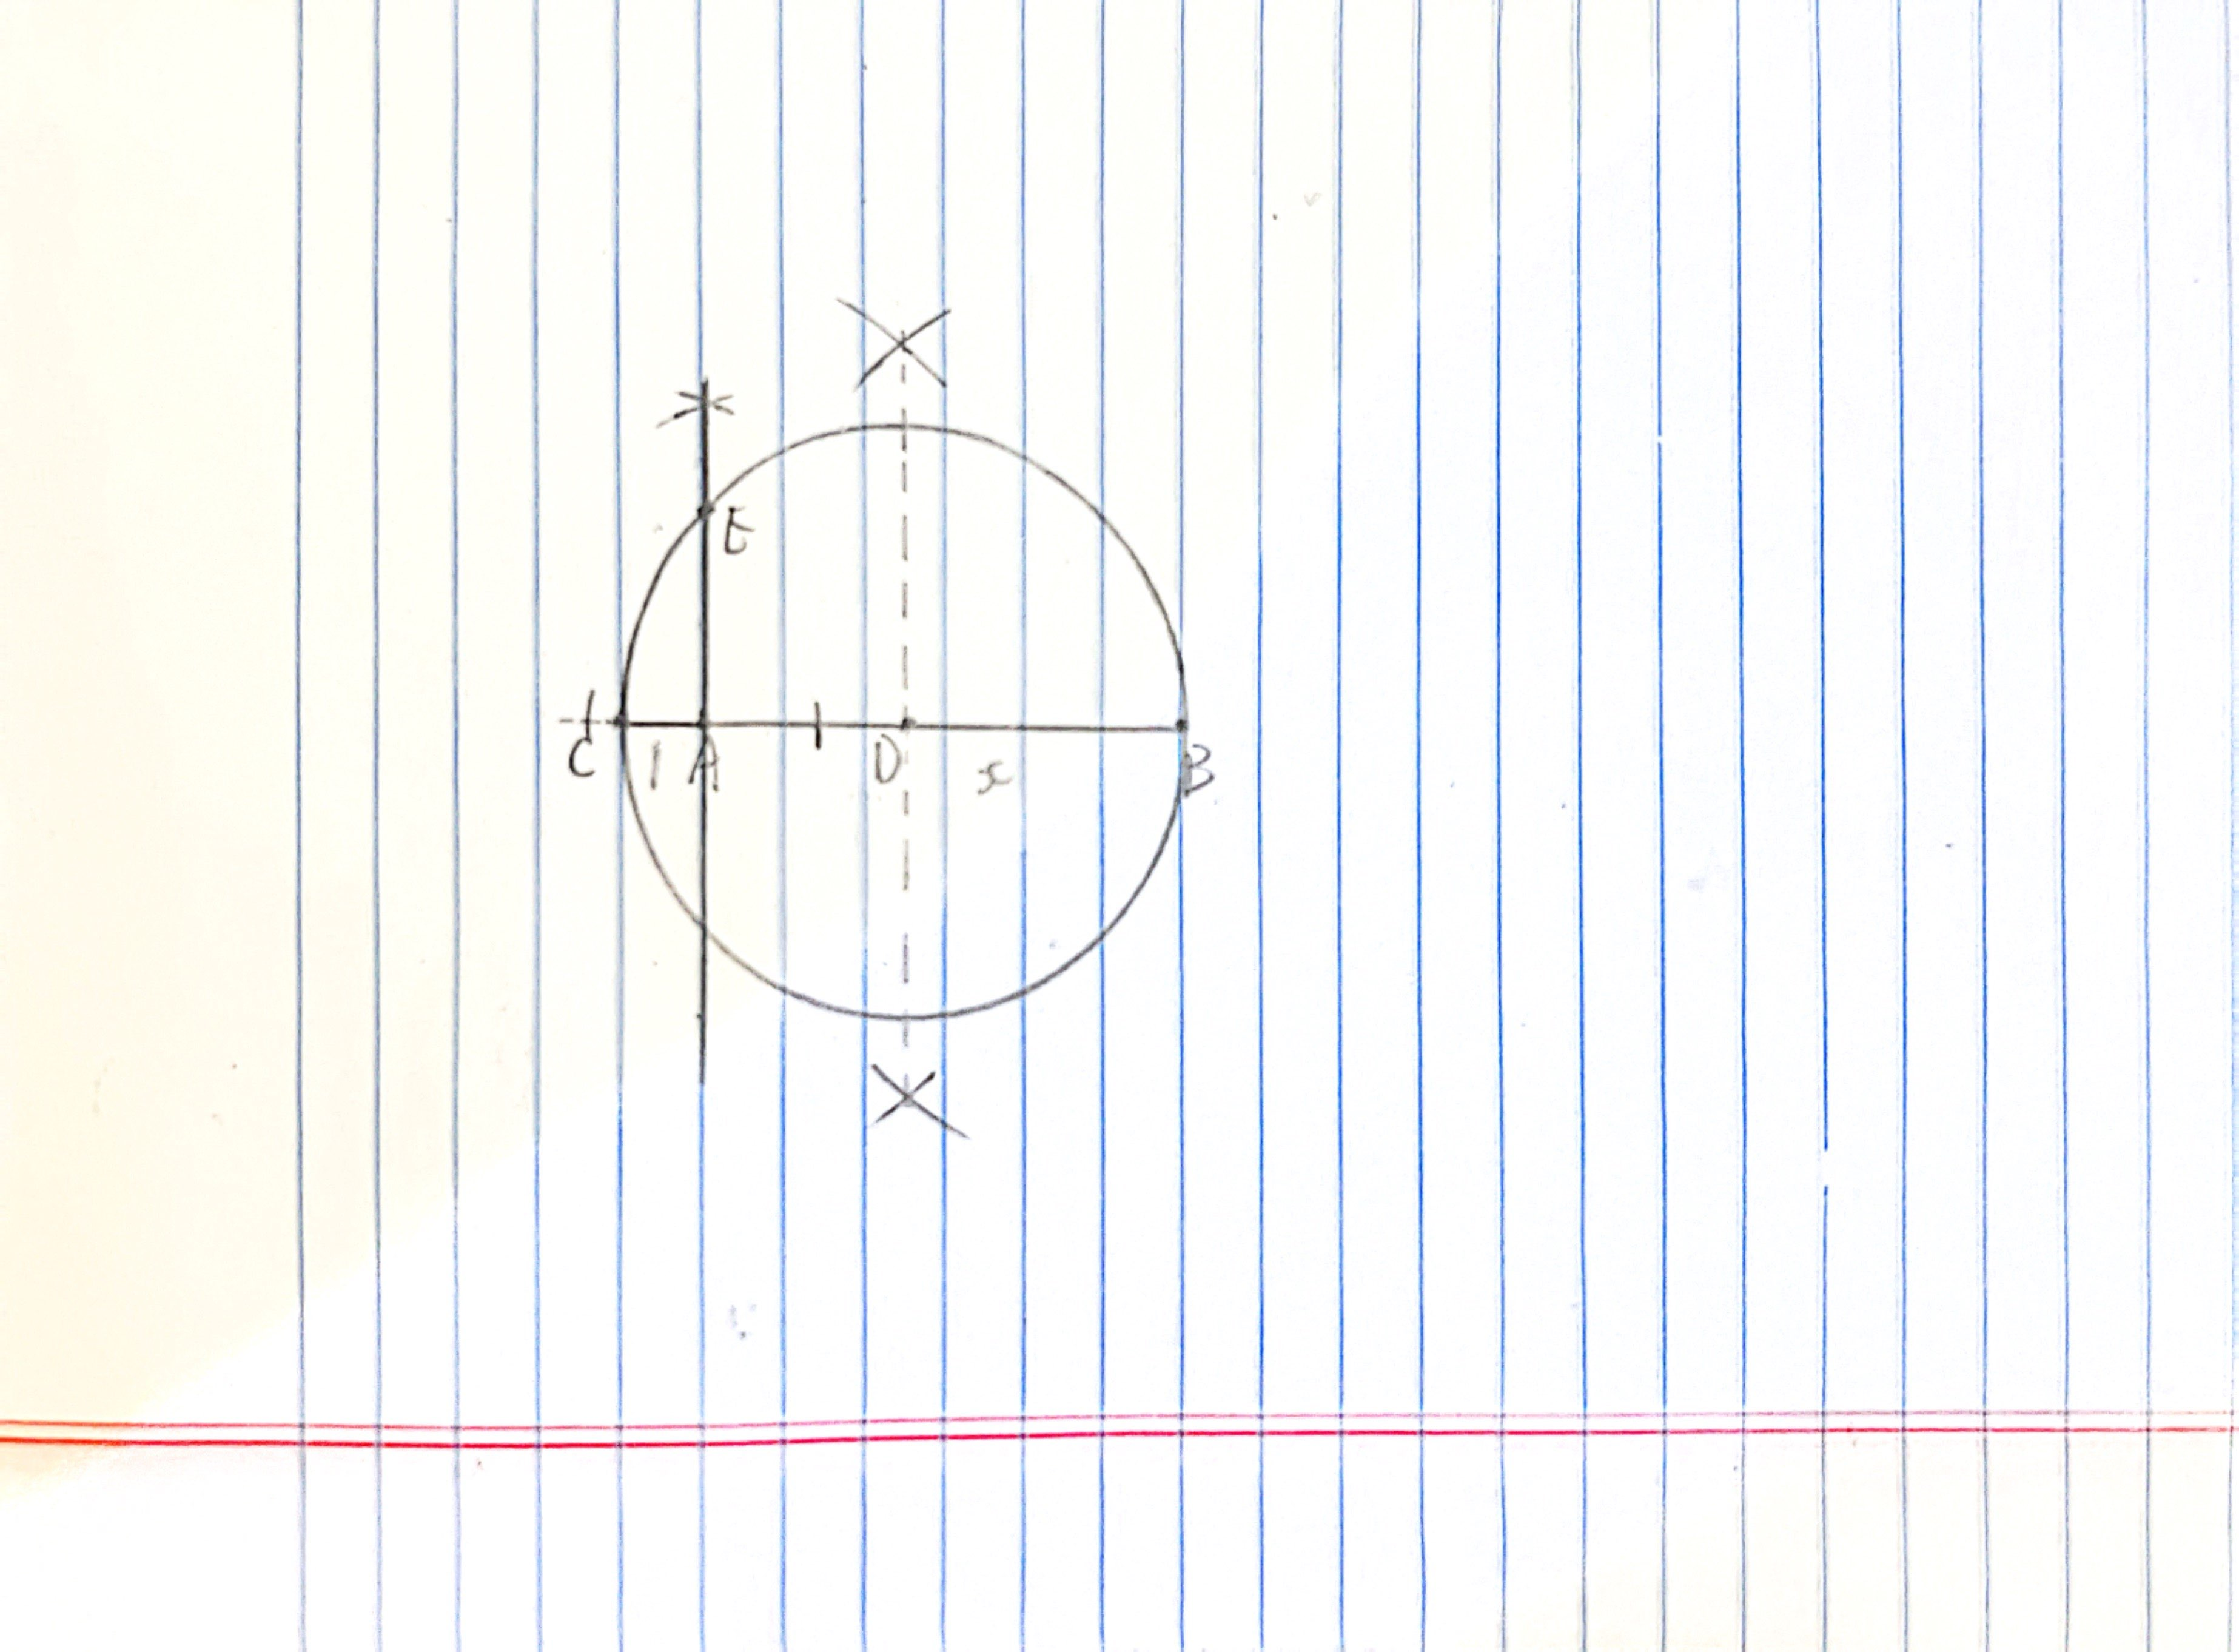
\includegraphics[scale=0.05]{HW_0214/cv_1.jpg}

\begin{proof}
    \begin{align*}
        &\text{Connects }OE\\
        \Rightarrow&OE=\frac{x+1}{2}\\
        &OA=OC-AC=\frac{x+1}{2}-1=\frac{x-1}{2}\\
        &AE\perp BC\\
        \Rightarrow&\Delta OAE \text{ is a right triangle}\\
        &OA^2+AE^2=OE^2\\
        &\left(\frac{x-1}{2}\right)^2+AE^2=\left(\frac{x+1}{2}\right)^2\\
        &\frac{x^2-2x+1}{4}+AE^2=\frac{x^2+2x+1}{4}\\
        &AE^2=x\\
        &AE=\sqrt{x}\ \ (\text{negative root is meaningless})\\
    \end{align*}
\end{proof}

\newpage

\section*{Question 4}

~

\subsection*{a}

~

\subsubsection*{i}

~

\begin{proof}
    \begin{align*}
        &\Delta ABC\text{ is isosceles by }AB=AC\\
        \Rightarrow&\angle ACB=\angle ABC\\
        &\angle BAC=36^\circ\land \angle ACB+\angle ABC+\angle BAC=180^\circ\\
        \Rightarrow&\angle ACB=\angle ABC=72^\circ\\
        &BE\text{ bisects }\angle ABC\\
        \Rightarrow& \angle CBE=36^\circ\\
        &\angle BEC=72^\circ\\
        \Rightarrow&\Delta BCE\text{ is isosceles by }BC=BE\\
        &\Delta ABC\text{ is similar to }\Delta BCE\\
        \Rightarrow&\frac{CE}{BC}=\frac{BC}{AC}\\
        &BE\text{ bisects }\angle ABC\\
        &\angle ABE=36^\circ\\
        \Rightarrow&\angle ABE=\angle BAE\\
        \Rightarrow&\Delta ABE\text{ is isosceles by }AE=BE\\
        &BC=AE\\
        \Rightarrow&\frac{CE}{AE}=\frac{AE}{AC}\\
        &CE:AE=AE:AC\\
    \end{align*}
\end{proof}

~

\subsubsection*{ii}

~

\begin{align*}
    &BC=AE\coloneqq x\\
    &CE=1-x\\
    \Rightarrow&\frac{1-x}{x}=\frac{x}{1}\\
    &x^2+x-1=0\\
    &x=\frac{\sqrt{5}-1}{2}(\text{the negative value is meaningless})\\
    \Rightarrow&BC=\frac{\sqrt{5}-1}{2}\\
\end{align*}

~

\subsubsection*{iii}

~

By connecting every vertex of the decagon to the center, there are 10 congruent isosceles triangles, making the acutest angle in the triangles $36^\circ$. So every triangle is similar to $\Delta ABC$. And with the radius 1, the ten triangles are all congruent to $\Delta ABC$, so the length of the side of the decagon should be the same as $BC$, $\frac{\sqrt{5}-1}{2}$.

~

\subsection*{b}

~

\subsubsection*{i}

~

\begin{align*}
    &\text{By construction}:\\
    &\angle EOB=90^\circ\\
    &OE=EF=\frac{1}{2}\\
    &OB=1\\
    &\text{Since }\Delta BOE\text{ is a right triangle}\\
    &BE=\sqrt{OE^2+OB^2}=\frac{\sqrt{5}}{2}\\
    &BF=BE-FE=\frac{\sqrt{5}-1}{2}\\
\end{align*}

~

\subsubsection*{ii}

~

Connect $BG$, $BG=BF=\frac{\sqrt{5}-1}{2}$, and $OB=OG=1$, so $\Delta BOG$ is congruent to the triangle $ABC$ in part a. So $\angle BOG=\angle BAC=36^\circ$\\

~

\subsubsection*{iii}

~

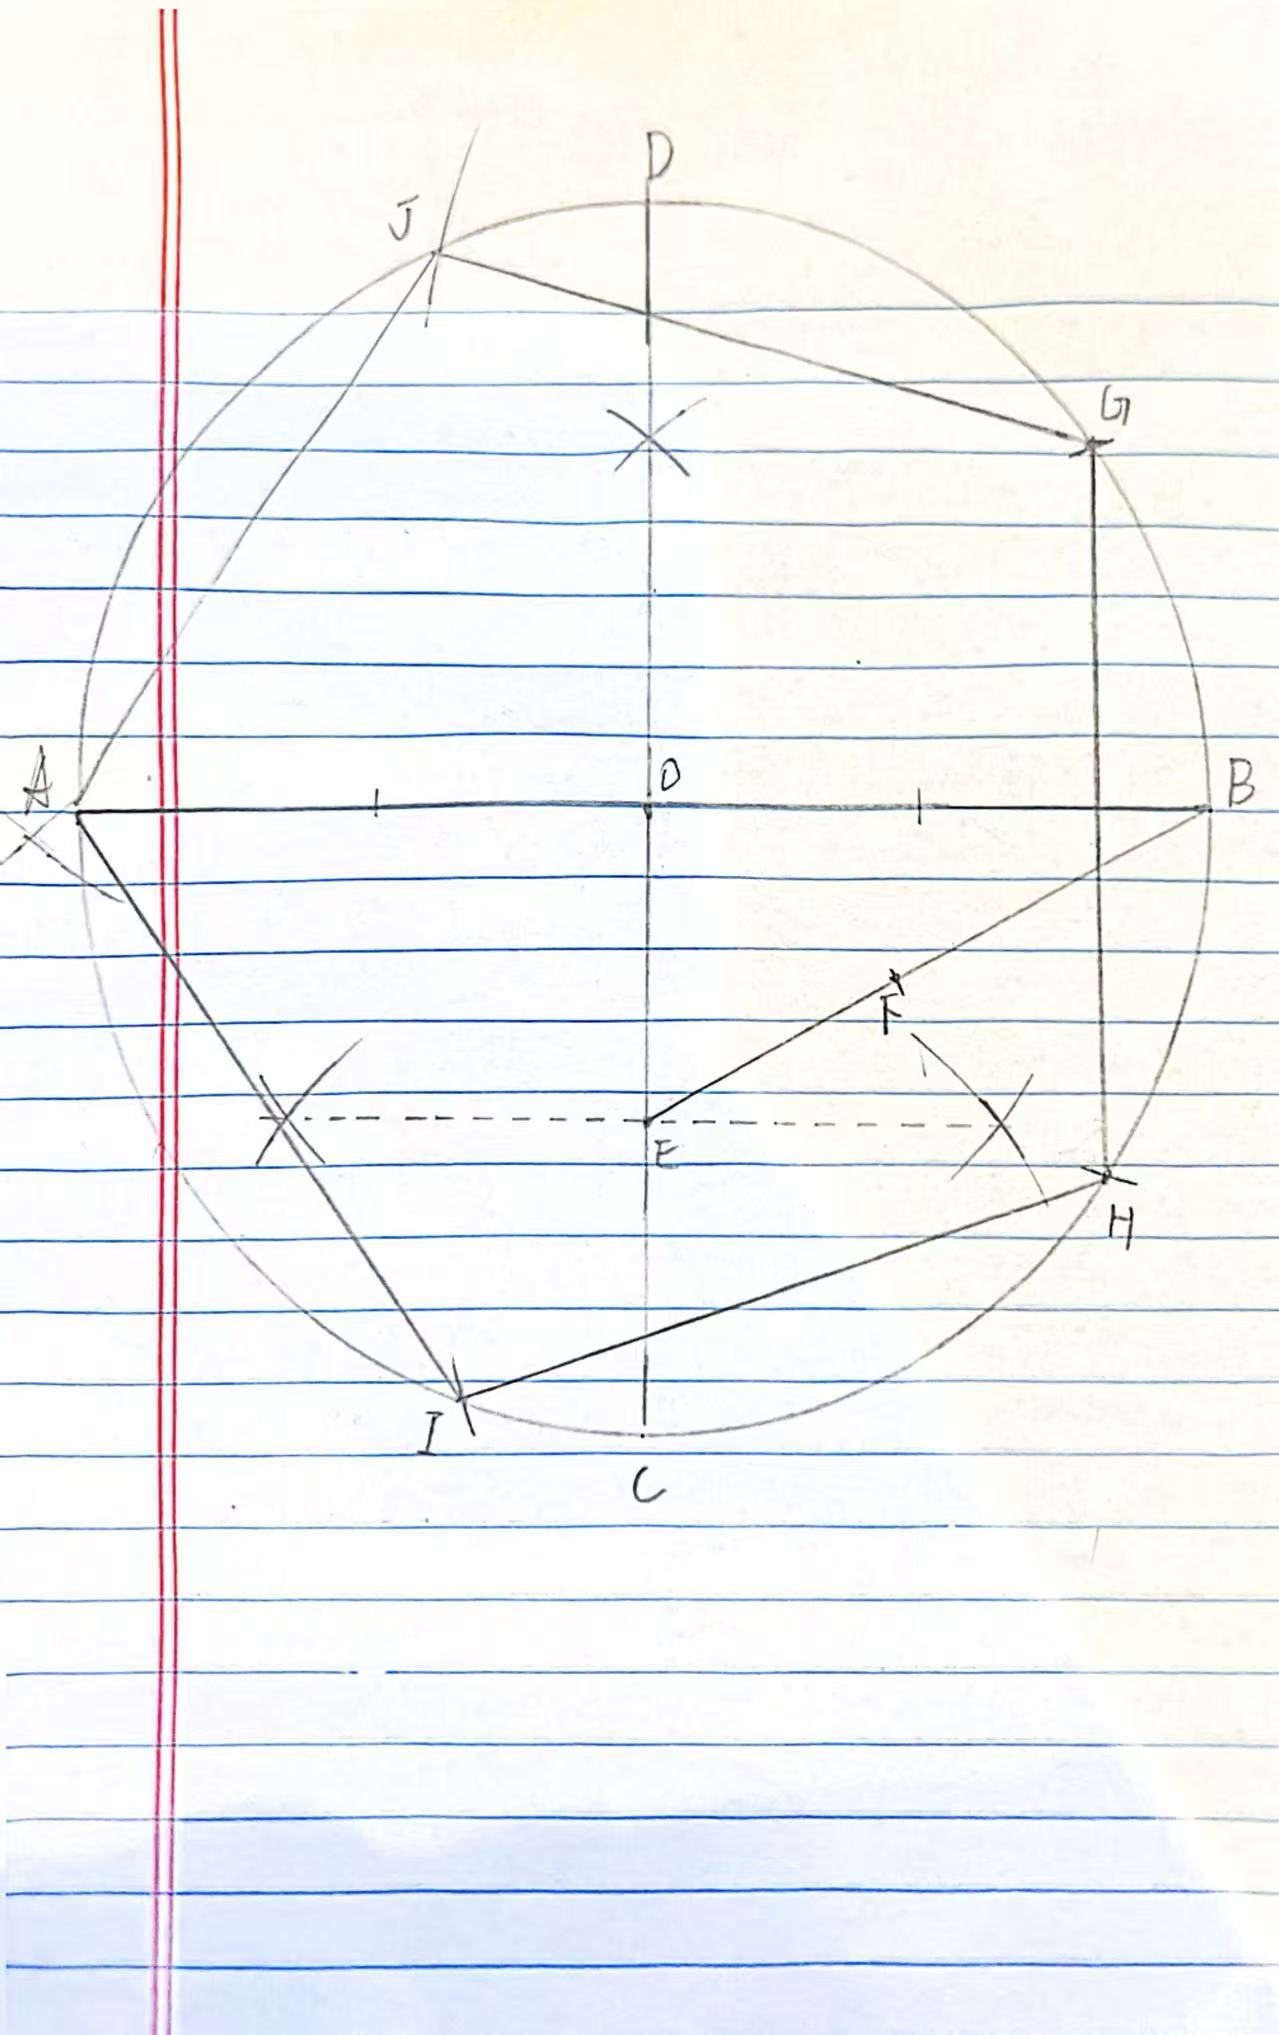
\includegraphics[scale=0.1]{HW_0214/4biii.jpg}

Use the steps up to ii to get $G$, then mark the other intersection of the circle $O$ and circle $B$ as $H$. Then draw an arc with center $H$ and radius $GH$ that intersects the circle with $I$ different than $G$. Draw an arc with center $G$ and radius $HG$ that intersects the circle with $J$ different than $H$. Then connect $AI, IH,HG,GJ,JA$. The pentagon $AIHGJ$ is a regular pentagon.

~

\subsection*{c}

~

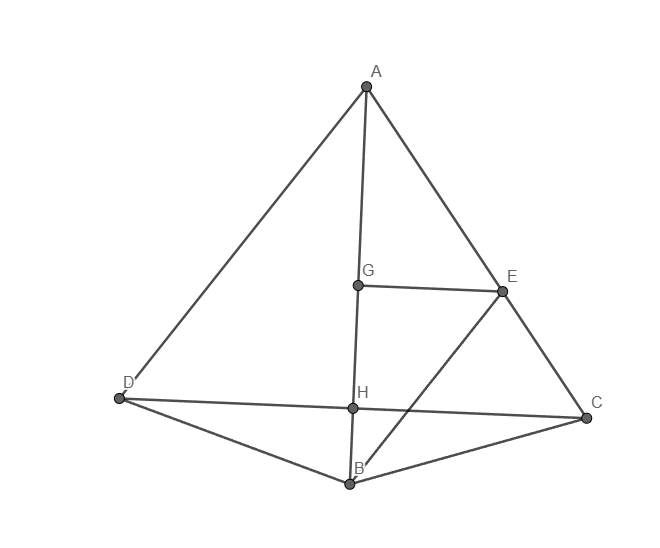
\includegraphics[scale=0.5]{HW_0214/4c.png}

$\Delta ABC$ is the same triangle described in 4(a). $\Delta ABD$ is $\Delta ABC$ reflected along $AB$. So $\angle CAD=72^\circ$ and $AD=AC$, making $CD$ the length of a regular pentagon inscribed in circle of radius 1. Since the coefficient given by the radius of the circle can be offset, only considering the circle with radius of 1 is efficient for the proof

\begin{proof}
    \begin{align*}
        &AB=AC=1\\
        &AE=BE=BC=\frac{\sqrt{5}-1}{2}\\
        &EG\text{ is perpendicular to }AB\\
        \Rightarrow&BG=\frac{1}{2}AB=0.5\\
        &CH=\sin 36^\circ\cdot AC=\sin 36^\circ\\
        &\sin36^\circ=\frac{GE}{BE}=\frac{\sqrt{BE^2-BG^2}}{BE}\\
        &=\frac{\sqrt{\left(\frac{\sqrt{5}-1}{2}\right)^2-\frac{1}{4}}}{\frac{\sqrt{5}-1}{2}}\\
        &=\frac{\sqrt{\frac{5-2\sqrt{5}}{4}}}{\frac{\sqrt{5}-1}{2}}\\
        &=\frac{\sqrt{5-2\sqrt{5}}}{\sqrt{5}-1}\\
        &=\frac{\sqrt{5-2\sqrt{5}}(\sqrt{5}+1)}{4}\\
        &=\frac{\sqrt{10-2\sqrt{5}}}{4}\\
        \Rightarrow&CH=\frac{\sqrt{10-2\sqrt{5}}}{4}\\
        &AD=AC\land \angle CAH=\frac{1}{2}\angle CAD\\
        \Rightarrow&CD=2CH=\frac{\sqrt{10-2\sqrt{5}}}{2}\\
        &\text{Side of a regular pentagon inscribed in circle of radius 1 is }\frac{\sqrt{10-2\sqrt{5}}}{2}\\
        &\text{hexagon}:\\
        &\text{the central angle formed by two near vertices is }60^\circ\\
        \Rightarrow&\text{The triangle formed by two near vertices and the center is equilateral}\\
        \Rightarrow&\text{Side length of regular hexagon inscribed in circle of radius 1 is } 1\\
        &\text{Side length of regular decagon inscribed in circle of radius 1 is } \frac{\sqrt{5}-1}{2}\\
        &S_{pentagon}=\frac{\sqrt{10-2\sqrt{5}}}{2}\\
        &S_{hexagon}=1\\
        &S_{decagon}=\frac{\sqrt{5}-1}{2}\\
        &{S_{decagon}}^2+{S_{hexagon}}^2=\left(\frac{\sqrt{5}-1}{2}\right)^2+1^2=\frac{5-\sqrt{5}}{2}\\
        &{S_{pentagon}}^2=\left(\frac{\sqrt{10-2\sqrt{5}}}{2}\right)^2=\frac{5-\sqrt{5}}{2}\\
        \Rightarrow&{S_{decagon}}^2+{S_{hexagon}}^2={S_{pentagon}}^2\\
    \end{align*}
\end{proof}

\newpage

\section*{Question 5}

~

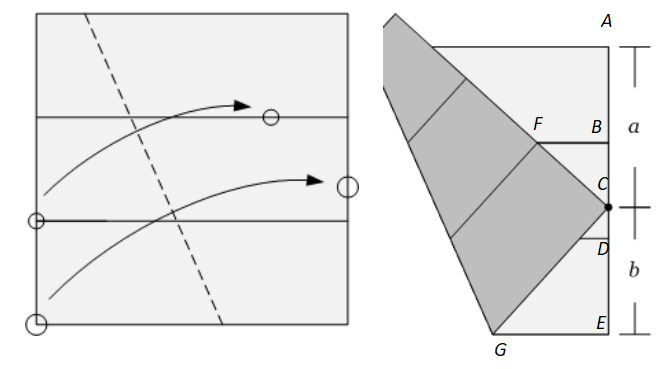
\includegraphics[scale=0.5]{HW_0214/5.png}


\begin{proof}
        \begin{align*}
        &EG\coloneqq x\\
        &CG+EG=a+1\\
        \Rightarrow&CG=a+1-x\\
        &\Delta CEG\text{ is right triangle}\\
        \Rightarrow&x^2+1^2=(a+1-x)^2\\
        &x^2+1=1+2a+a^2-2x-2ax+x^2\\
        &(2a+2)x=a^2+2a\\
        &x=\frac{a^2+2a}{2a+2}\\
        \Rightarrow&EG=\frac{a^2+2a}{2a+2}\\
        &BC=a-\frac{1}{3}(a+1)=\frac{2}{3}a-\frac{1}{3}\\
        &CF=\frac{1}{3}(a+1)\\
        &\Delta BCF\text{ is right triangle}\\
        \Rightarrow&BF=\sqrt{\left(\frac{1}{3}(a+1)\right)^2-\left(\frac{2}{3}a-\frac{1}{3}\right)^2}\\
        &=\frac{\sqrt{6a-3a^2}}{3}\\
        &\angle BCF+\angle GCE+90^\circ=180^\circ\\
        &\angle CGE+\angle GCE+90^\circ=180^\circ\\
        \Rightarrow&\angle BCF=\angle CGE\\
        &\angle CBF=\angle GEC=90^\circ\\
        &\text{So }\Delta BCF\text{ and }\Delta EGC \text{ are similar}\\
        \Rightarrow&\frac{EG}{CE}=\frac{BC}{BF}\\
        &\frac{a^2+2a}{2a+2}=\frac{\frac{2}{3}a-\frac{1}{3}}{\frac{\sqrt{6a-3a^2}}{3}}\\
        &(a^2+2a)\sqrt{6a-3a^2}=(2a+2)(2a-1)\\
        &(a^2+2a)^2(6a-3a^2)=((2a+2)(2a-1))^2\\
        &-3a^6-6a^5+12a^4+24a^3=16a^4+16a^3-12a^2-8a-4\\
        &3a^6+6a^5+4a^4-8a^3-12a^2-8a+4=0\\
        &(a^3-2)(3a^3+6a^2+4a-2)=0\\
        &a=\sqrt[3]{2}\\
        \Rightarrow&\frac{a}{b}=\sqrt[3]{2}\\
    \end{align*}
\end{proof}
\end{document}